\documentclass[10pt, letterpaper]{article}

% Inhaltsverzeichnis für Pakettypen (nur für Übersicht im Header, wird nicht im Dokument angezeigt)
% 1. Seitenlayout und Ränder
% 2. Sprache und Zeichensatz
% 3. Mathematik und Theorem-Umgebungen
% 4. Eigene Makros
% 5. Diagramme und Grafiken
% 6. Tabellen und Aufzählungen
% 7. Inhaltsverzeichnis
% 8. Abschnittsüberschriften
% 9. Abstrakt-Umgebung
% 10. Todos/Notizen
% 11. Rahmen/Box-Umgebungen
% 12. Python-Integration
% 13. Literaturverwaltung
% 14. Hyperlinks
% 15. Absatzeinstellungen
% 16. Umgebungen
% 17  Graphik
% 18  Extra
% 00. Titel und Autor

% --- 1. Seitenlayout und Ränder ---
\usepackage[margin=3cm]{geometry}

% --- 2. Sprache und Zeichensatz ---
\usepackage[english]{babel}
\usepackage[T1]{fontenc}
\usepackage[utf8]{inputenc}

% --- 3. Mathematik und Theorem-Umgebungen ---
\usepackage{amsmath, amssymb, amsthm}
\usepackage{mathrsfs}
\DeclareMathOperator{\WF}{WF}

% --- 4. Eigene Makros ---
\usepackage{xcolor}
\newcommand{\SKP}{\langle\cdot,\cdot\rangle}
\newcommand{\R}{\mathbb{R}}
\newcommand{\N}{\mathbb{N}}
\newcommand{\Q}{\mathbb{Q}}
\newcommand{\Z}{\mathbb{Z}}
\newcommand{\C}{\mathbb{C}}
\newcommand{\entwurf}[1]{\textcolor{red}{#1}}

% --- 5. Diagramme und Grafiken ---
\usepackage{graphicx}
\usepackage{tikz}
\usetikzlibrary{decorations.pathreplacing, arrows.meta, positioning}
\usepackage{tikz-cd}

% --- 6. Tabellen und Aufzählungen ---
\usepackage{enumitem}
\setlist[itemize]{left=0.5cm}

\newenvironment{romanenum}[1][]
  {%
    \ifx&#1&
    \else
      \textbf{#1}\quad
    \fi
    \begin{enumerate}[label=\roman*)]
  }
  {%
    \end{enumerate}%
  }

% --- 7. Inhaltsverzeichnis ---
\usepackage{tocloft}
\renewcommand{\cftsecfont}{\footnotesize}
\renewcommand{\cftsubsecfont}{\footnotesize}
\renewcommand{\cftsubsubsecfont}{\footnotesize}
\renewcommand{\cftsecpagefont}{\footnotesize}
\renewcommand{\cftsubsecpagefont}{\footnotesize}
\renewcommand{\cftsubsubsecpagefont}{\footnotesize}
\usepackage{etoc}

% --- 8. Abschnittsüberschriften ---
\usepackage{titlesec}
\titleformat{\section}{\normalfont\large\bfseries}{\thesection}{1em}{}
\titleformat{\subsection}{\normalfont\normalsize\bfseries}{\thesubsection}{0.5em}{}
\titleformat{\subsubsection}{\normalfont\normalsize\bfseries}{\thesubsubsection}{0.5em}{}
\setcounter{secnumdepth}{4}

% --- 9. Abstrakt-Umgebung ---
\usepackage{changepage}
\renewenvironment{abstract}
  {
    \begin{adjustwidth}{1.5cm}{1.5cm}
    \small
    \textsc{Abstract. –}%
  }
  {
    \end{adjustwidth}
  }

% --- 10. Todos/Notizen ---
\usepackage{todonotes}

% --- 11. Rahmen/Box-Umgebungen ---
\usepackage{mdframed}
\usepackage{tcolorbox}
\colorlet{shadecolor}{gray!25}

\newenvironment{customTheorem}
  {\vspace{10pt}%
   \begin{mdframed}[
     backgroundcolor=gray!20,
     linewidth=0pt,
     innertopmargin=10pt,
     innerbottommargin=10pt,
     skipabove=\dimexpr\topsep+\ht\strutbox\relax,
     skipbelow=\topsep,
   ]}
  {\end{mdframed}
   \vspace{10pt}%
  }

% --- 12. Python-Integration ---
% (Deaktiviert in dieser Version, aktiviere bei Bedarf)
% \usepackage{pythontex}
% \usepackage[makestderr]{pythontex}

% --- 13. Literaturverwaltung ---
\usepackage{csquotes}
\usepackage[backend=biber, style=alphabetic, citestyle=alphabetic]{biblatex}
\addbibresource{bibliography.bib}

% --- 14. Hyperlinks ---
\usepackage{hyperref}
\hypersetup{
  colorlinks   = true,
  urlcolor     = blue,
  linkcolor    = blue,
  citecolor    = blue,
  frenchlinks  = true
}

% --- 15. Absatzeinstellungen ---
\usepackage[parfill]{parskip}
\sloppy

% --- 16. Umgebungen ---
\usepackage{thmtools}

\newcommand{\CustomHeading}[3]{%
  \par\medskip\noindent%
  \textbf{#1 #2} \textnormal{(#3)}.\enskip%
}

\newenvironment{DEF}[2]{\begin{unitbox}\CustomHeading{Definition}{#1}{#2}}{\end{unitbox}}
\newenvironment{PROP}[2]{\begin{unitbox}\CustomHeading{Proposition}{#1}{#2}}{\end{unitbox}}
\newenvironment{THEO}[2]{\begin{unitbox}\CustomHeading{Theorem}{#1}{#2}}{\end{unitbox}}
\newenvironment{LEM}[2]{\begin{unitbox}\CustomHeading{Lemma}{#1}{#2}}{\end{unitbox}}
\newenvironment{KORO}[2]{\begin{unitbox}\CustomHeading{Corollar}{#1}{#2}}{\end{unitbox}}
\newenvironment{REM}[2]{\begin{unitbox}\CustomHeading{Remark}{#1}{#2}}{\end{unitbox}}
\newenvironment{EXA}[2]{\begin{unitbox}\CustomHeading{Example}{#1}{#2}}{\end{unitbox}}
\newenvironment{STUD}[2]{\begin{unitbox}\CustomHeading{Study}{#1}{#2}}{\end{unitbox}}
\newenvironment{CONC}[2]{\begin{unitbox}\CustomHeading{Concept}{#1}{#2}}{\end{unitbox}}
\newenvironment{OTH}[2]{\begin{unitbox}\CustomHeading{Other}{#1}{#2}}{\end{unitbox}}
\newenvironment{EXE}[2]{\begin{unitbox}\CustomHeading{Exercise}{#1}{#2}}{\end{unitbox}}
\newenvironment{MOT}[2]{\begin{unitbox}\CustomHeading{Motivation}{#1}{#2}}{\end{unitbox}}
\newenvironment{PROOF}[2]{\begin{unitbox}\CustomHeading{Proof}{#1}{#2}}{\end{unitbox}}

% --- Unit Umgebung für Source-Inhalte ---
\usepackage{mdframed}
\newmdenv[
  linewidth=1pt,
  topline=false,
  bottomline=false,
  rightline=false,
  leftmargin=0cm,
  rightmargin=0cm,
  skipabove=10pt,
  skipbelow=10pt,
  innertopmargin=0.5\baselineskip,
  innerbottommargin=0.5\baselineskip,
  backgroundcolor=gray!10,
  linecolor=gray
]{unitbox}

\newenvironment{unit}[1]
  {\begin{unitbox}\textbf{Unit #1}\par\smallskip}
  {\end{unitbox}}

% --- 17. Graphik ---
\usepackage{graphicx}
\graphicspath{ {./images/} }
\usepackage[export]{adjustbox}

% --- 18. Extras ---
\usepackage{stmaryrd}
\usepackage{bbold}  % falls du athbb{1} nutzen willst

% --- 00. Titel und Autor ---
\title{Mein Titel}
\author{Tim Jaschik}
\date{\today}


%New command to display footnote whose markers will always be hidden
\let\svthefootnote\thefootnote
\newcommand\blfootnotetext[1]{%
  \let\thefootnote\relax\footnote{#1}%
  \addtocounter{footnote}{-1}%
  \let\thefootnote\svthefootnote%
}

%Overriding the \footnotetext command to hide the marker if its value is `0`
\let\svfootnotetext\footnotetext
\renewcommand\footnotetext[2][?]{%
  \if\relax#1\relax%
    \ifnum\value{footnote}=0\blfootnotetext{#2}\else\svfootnotetext{#2}\fi%
  \else%
    \if?#1\ifnum\value{footnote}=0\blfootnotetext{#2}\else\svfootnotetext{#2}\fi%
    \else\svfootnotetext[#1]{#2}\fi%
  \fi
}


\begin{document}

\maketitle
\rule{\textwidth}{0.5pt}
\begin{abstract}
Kurze Beschreibung …
\end{abstract}
\rule{\textwidth}{0.5pt}
\vspace{0.5cm}

\tableofcontents

\pagebreak


\section*{§1. SMOOTH MANIFOLDS AND SMOOTH MAPS}


First let us explain some of our terms. $R^{k}$ denotes the $k$-dimensional euclidean space; thus a point $x \in R^{k}$ is an $k$-tuple $x=\left(x_{1}, \cdots, x_{k}\right)$ of real numbers.

Let $U \subset R^{k}$ and $V \subset R^{l}$ be open sets. A mapping $f$ from $U$ to $V$ (written $f: U \rightarrow V$ ) is called smooth if all of the partial derivatives $\partial^{n} f / \partial x_{i_{1}} \cdots \partial x_{i_{n}}$ exist and are continuous.

More generally let $X \subset R^{k}$ and $Y \subset R^{l}$ be arbitrary subsets of euclidean spaces. A map $f: X \rightarrow Y$ is called smooth if for each $x \in X$ there exist an open set $U \subset R^{k}$ containing $x$ and a smooth mapping $F: U \rightarrow R^{l}$ that coincides with $f$ throughout $U \cap X$.

If $f: X \rightarrow Y$ and $g: Y \rightarrow Z$ are smooth, note that the composition $g \circ f: X \rightarrow Z$ is also smooth. The identity map of any set $X$ is automatically smooth.

Definition. A map $f: X \rightarrow Y$ is called a diffeomorphism if $f$ carries $X$ homeomorphically onto $Y$ and if both $f$ and $f^{-1}$ are smooth.

We can now indicate roughly what differential topology is about by saying that it studies those properties of a set $X \subset R^{k}$ which are invariant under diffeomorphism.

We do not, however, want to look at completely arbitrary sets $X$. The following definition singles out a particularly attractive and useful class.

Definition. A subset $M \subset R^{k}$ is called a smooth manifold of dimension $m$ if each $x \in M$ has a neighborhood $W \cap M$ that is diffeomorphic to an open subset $U$ of the euclidean space $R^{m}$.

Any particular diffeomorphism $g: U \rightarrow W \cap M$ is called a parametrization of the region $W \cap M$. (The inverse diffeomorphism $W \cap M \rightarrow U$ is called a system of coordinates on $W \cap M$.)\\
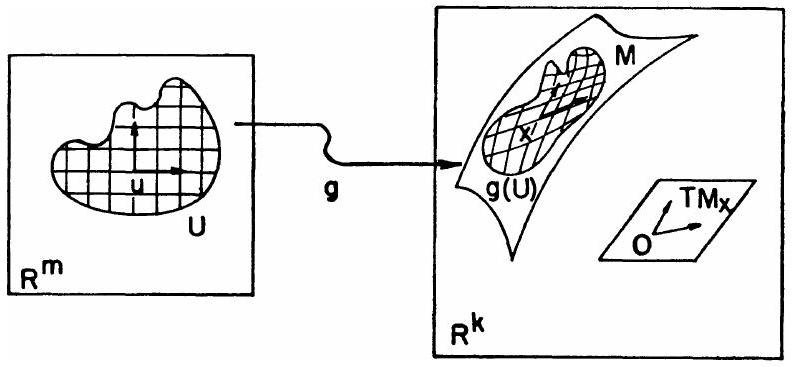
\includegraphics[scale=0.2, center]{2025_05_28_7c9927389b272ddbc2c3g-13}

Figure 1. Parametrization of a region in $M$

Sometimes we will need to look at manifolds of dimension zero. By definition, $M$ is a manifold of dimension zero if each $x \varepsilon M$ has a neighborhood $W \cap M$ consisting of $x$ alone.

Examples. The unit sphere $S^{2}$, consisting of all $(x, y, z) \varepsilon R^{3}$ with $x^{2}+y^{2}+z^{2}=1$ is a smooth manifold of dimension 2 . In fact the diffeomorphism

$$
(x, y) \rightarrow\left(x, y, \sqrt{1-x^{2}-y^{2}}\right)
$$

for $x^{2}+y^{2}<1$, parametrizes the region $z>0$ of $S^{2}$. By interchanging the roles of $x, y, z$, and changing the signs of the variables, we obtain similar parametrizations of the regions $x>0, y>0, x<0, y<0$, and $z<0$. Since these cover $S^{2}$, it follows that $S^{2}$ is a smooth manifold.

More generally the sphere $S^{n-1} \subset R^{n}$ consisting of all ( $x_{1}, \cdots, x_{n}$ ) with $\sum x_{i}^{2}=1$ is a smooth manifold of dimension $n-1$. For example $S^{0} \subset R^{1}$ is a manifold consisting of just two points.

A somewhat wilder example of a smooth manifold is given by the set of all $(x, y) \varepsilon R^{2}$ with $x \neq 0$ and $y=\sin (1 / x)$.

\section*{TANGENT SPACES AND DERIVATIVES}
To define the notion of derivative $d f_{x}$ for a smooth map $f: M \rightarrow N$ of smooth manifolds, we first associate with each $x \varepsilon M \subset R^{k}$ a linear subspace $T M_{x} \subset R^{k}$ of dimension $m$ called the tangent space of $M$ at $x$. Then $d f_{x}$ will be a linear mapping from $T M_{x}$ to $T N_{y}$, where $y=f(x)$. Elements of the vector space $T M_{x}$ are called tangent vectors to $M$ at $x$.

Intuitively one thinks of the $m$-dimensional hyperplane in $R^{k}$ which best approximates $M$ near $x$; then $T M_{x}$ is the hyperplane through the\\
origin that is parallel to this. (Compare Figures 1 and 2.) Similarly one thinks of the nonhomogeneous linear mapping from the tangent hyperplane at $x$ to the tangent hyperplane at $y$ which best approximates $f$. Translating both hyperplanes to the origin, one obtains $d f_{x}$.

Before giving the actual definition, we must study the special case of mappings between open sets. For any open set $U \subset R^{k}$ the tangent space $T U_{x}$ is defined to be the entire vector space $R^{k}$. For any smooth map $f: U \rightarrow V$ the derivative

$$
d f_{x}: R^{k} \rightarrow R^{l}
$$

is defined by the formula

$$
d f_{x}(h)=\lim _{t \rightarrow 0}(f(x+t h)-f(x)) / t
$$

for $x \varepsilon U, h \varepsilon R^{k}$. Clearly $d f_{x}(h)$ is a linear function of $h$. (In fact $d f_{x}$ is just that linear mapping which corresponds to the $l \times k$ matrix $\left(\partial f_{i} / \partial x_{i}\right)_{x}$ of first partial derivatives, evaluated at $x$.)

Here are two fundamental properties of the derivative operation:\\
1 (Chain rule). If $f: U \rightarrow V$ and $g: V \rightarrow W$ are smooth maps, with $f(x)=y$, then

$$
d(g \circ f)_{x}=d g_{y} \circ d f_{x} .
$$

In other words, to every commutative triangle\\
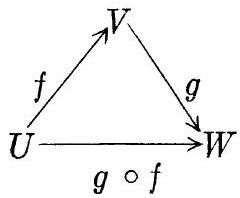
\includegraphics[scale=0.2, center]{2025_05_28_7c9927389b272ddbc2c3g-14(1)}\\
of smooth maps between open subsets of $R^{k}, R^{l}, R^{m}$ there corresponds a commutative triangle of linear maps\\
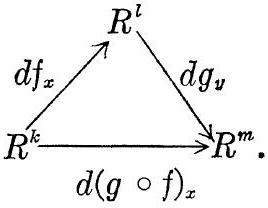
\includegraphics[scale=0.2, center]{2025_05_28_7c9927389b272ddbc2c3g-14}\\
2. If $I$ is the identity map of $U$, then $d I_{x}$ is the identity map of $R^{k}$. More generally, if $U \subset U^{\prime}$ are open sets and

$$
i: U \rightarrow U^{\prime}
$$

is the inclusion map, then again di ${ }_{x}$ is the identity map of $R^{k}$.\\
Note also:\\
3. If $L: R^{k} \rightarrow R^{l}$ is a linear mapping, then $d L_{x}=L$.

As a simple application of the two properties one has the following:\\
Assertion. If $f$ is a diffeomorphism between open sets $U \subset R^{k}$ and $V \subset R^{l}$, then $k$ must equal $l$, and the linear mapping

$$
d f_{x}: R^{k} \rightarrow R^{l}
$$

must be nonsingular.\\
Proof. The composition $f^{-1} \circ f$ is the identity map of $U$; hence $d\left(f^{-1}\right)_{y} \circ d f_{x}$ is the identity map of $R^{k}$. Similarly $d f_{x} \circ d\left(f^{-1}\right)_{y}$ is the identity map of $R^{l}$. Thus $d f_{x}$ has a two-sided inverse, and it follows that $k=l$.

A partial converse to this assertion is valid. Let $f: U \rightarrow R^{k}$ be a smooth map, with $U$ open in $R^{k}$.

Inverse Function Theorem. If the derivative $d f_{x}: R^{k} \rightarrow R^{k}$ is nonsingular, then $f$ maps any sufficiently small open set $U^{\prime}$ about $x$ diffeomorphically onto an open set $f\left(U^{\prime}\right)$.\\[0pt]
(See Apostol [2, p. 144] or Dieudonné [7, p. 268].)\\
Note that $f$ may not be one-one in the large, even if every $d f_{x}$ is nonsingular. (An instructive example is provided by the exponential mapping of the complex plane into itself.)

Now let us define the tangent space $T M_{x}$ for an arbitrary smooth manifold $M \subset R^{k}$. Choose a parametrization

$$
g: U \rightarrow M \subset R^{k}
$$

of a neighborhood $g(U)$ of $x$ in $M$, with $g(u)=x$. Here $U$ is an open subset of $R^{m}$. Think of $g$ as a mapping from $U$ to $R^{k}$, so that the derivative

$$
d g_{u}: R^{m} \rightarrow R^{k}
$$

is defined. Set $T M_{x}$ equal to the image $d g_{u}\left(R^{m}\right)$ of $d g_{u}$. (Compare Figure 1.)\\
We must prove that this construction does not depend on the particular choice of parametrization $g$. Let $h: V \rightarrow M \subset R^{k}$ be another parametrization of a neighborhood $h(V)$ of $x$ in $M$, and let $v=h^{-1}(x)$. Then $h^{-1} \circ g$ maps some neighborhood $U_{1}$ of $u$ diffeomorphically onto a neighborhood $V_{1}$ of $v$. The commutative diagram of smooth maps\\
ween open sets\\
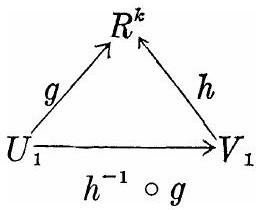
\includegraphics[scale=0.2, center]{2025_05_28_7c9927389b272ddbc2c3g-16(2)}\\
es rise to a commutative diagram of linear maps\\
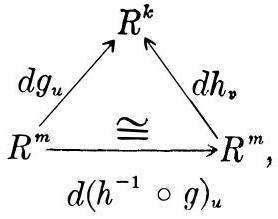
\includegraphics[scale=0.2, center]{2025_05_28_7c9927389b272ddbc2c3g-16(1)}

I it follows immediately that

$$
\text { Image }\left(d g_{u}\right)=\text { Image }\left(d h_{v}\right) .
$$

us $T M_{x}$ is well defined.\\
'roof that $T M_{x}$ is an $m$-dimensional vector space. Since

$$
g^{-1}: g(U) \rightarrow U
$$

, smooth mapping, we can choose an open set $W$ containing $x$ and mooth map $F: W \rightarrow R^{m}$ that coincides with $g^{-1}$ on $W \cap g(U)$. ting $U_{0}=g^{-1}(W \cap g(U))$, we have the commutative diagram\\
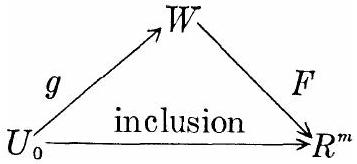
\includegraphics[scale=0.2, center]{2025_05_28_7c9927389b272ddbc2c3g-16(3)}\\
therefore\\
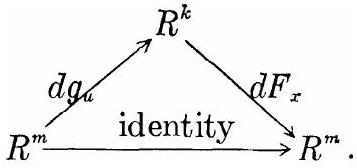
\includegraphics[scale=0.2, center]{2025_05_28_7c9927389b272ddbc2c3g-16}\\
s diagram clearly implies that $d g_{u}$ has rank $m$, and hence that its ge $T M_{x}$ has dimension $m$.\\
low consider two smooth manifolds, $M \subset R^{k}$ and $N \subset R^{l}$, and a\\
smooth map

$$
f: M \rightarrow N
$$

with $f(x)=y$. The derivative

$$
d f_{x}: T M_{x} \rightarrow T N_{y}
$$

is defined as follows. Since $f$ is smooth there exist an open set $W$ containing $x$ and a smooth map

$$
F: W \rightarrow R^{l}
$$

that coincides with $f$ on $W \cap M$. Define $d f_{x}(v)$ to be equal to $d F_{x}(v)$ for all $v \varepsilon T M_{x}$.

To justify this definition we must prove that $d F_{x}(v)$ belongs to $T N_{y}$ and that it does not depend on the particular choice of $F$.

Choose parametrizations

$$
g: U \rightarrow M \subset R^{k} \quad \text { and } \quad h: V \rightarrow N \subset R^{l}
$$

for neighborhoods $g(U)$ of $x$ and $h(V)$ of $y$. Replacing $U$ by a smaller set if necessary, we may assume that $g(U) \subset W$ and that $f$ maps $g(U)$ into $h(V)$. It follows that

$$
h^{-1} \circ f \circ g: U \rightarrow V
$$

is a well-defined smooth mapping.\\
Consider the commutative diagram\\
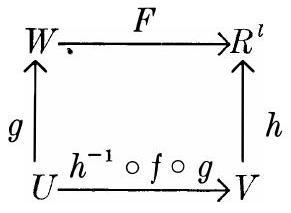
\includegraphics[scale=0.2, center]{2025_05_28_7c9927389b272ddbc2c3g-17(1)}\\
of smooth mappings between open sets. Taking derivatives, we obtain a commutative diagram of linear mappings\\
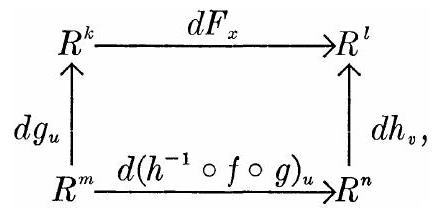
\includegraphics[scale=0.2, center]{2025_05_28_7c9927389b272ddbc2c3g-17}\\
where $u=g^{-1}(x), v=h^{-1}(y)$.\\
It follows immediately that $d F_{x}$ carries $T M_{x}=$ Image ( $d g_{u}$ ) into $T N_{y}=$ Image $\left(d h_{v}\right)$. Furthermore the resulting map $d f_{x}$ does not depend on the particular choice of $F$, for we can obtain the same linear\\
transformation by going around the bottom of the diagram. That is:

$$
d f_{x}=d h_{v} \circ d\left(h^{-1} \circ f \circ g\right)_{u} \circ\left(d g_{u}\right)^{-1} .
$$

This completes the proof that

$$
d f_{x}: T M_{x} \rightarrow T N_{y}
$$

is a well-defined linear mapping.\\
As before, the derivative operation has two fundamental properties:

\begin{enumerate}
  \item (Chain rule). If $f: M \rightarrow N$ and $g: N \rightarrow P$ are smooth, with $f(x)=y$, then
\end{enumerate}

$$
d(g \circ f)_{x}=d g_{y} \circ d f_{x} .
$$

\begin{enumerate}
  \setcounter{enumi}{1}
  \item If $I$ is the identity map of $M$, then $d I_{x}$ is the identity map of $T M_{x}$. More generally, if $M \subset N$ with inclusion map $i$, then $T M_{x} \subset T N_{x}$ with inclusion map di ${ }_{x}$. (Compare Figure 2.)\\
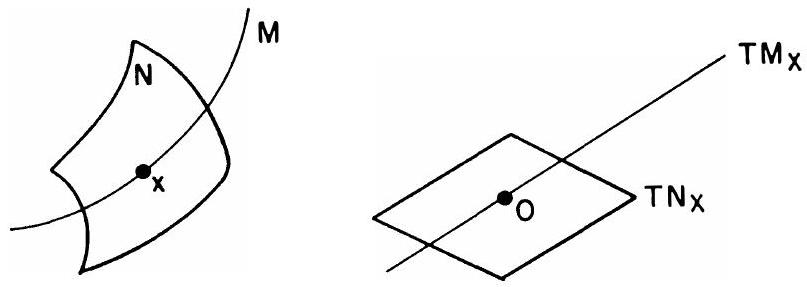
\includegraphics[scale=0.2, center]{2025_05_28_7c9927389b272ddbc2c3g-18}
\end{enumerate}

Figure 2. The tangent space of a submanifold

The proofs are straightforward.\\
As before, these two properties lead to the following:\\
Assertion. If $f: M \rightarrow N$ is a diffeomorphism, then $d f_{x}: T M_{x} \rightarrow T N_{y}$ is an isomorphism of vector spaces. In particular the dimension of $M$ must be equal to the dimension of $N$.

\section*{REGULAR VALUES}
Let $f: M \rightarrow N$ be a smooth map between manifolds of the same dimension.* We say that $x \in M$ is a regular point of $f$ if the derivative

\footnotetext{\begin{itemize}
  \item This restriction will be removed in §2.
\end{itemize}
}
$d f_{x}$ is nonsingular. In this case it follows from the inverse function theorem that $f$ maps a neighborhood of $x$ in $M$ diffeomorphically onto an open set in $N$. The point $y \varepsilon N$ is called a regular value if $f^{-1}(y)$ contains only regular points.

If $d f_{x}$ is singular, then $x$ is called a critical point of $f$, and the image $f(x)$ is called a critical value. Thus each $y \varepsilon N$ is either a critical value or a regular value according as $f^{-1}(y)$ does or does not contain a critical point.

Observe that if $M$ is compact and $y \varepsilon N$ is a regular value, then $f^{-1}(y)$ is a finite set (possibly empty). For $f^{-1}(y)$ is in any case compact, being a closed subset of the compact space $M$; and $f^{-1}(y)$ is discrete, since $f$ is one-one in a neighborhood of each $x \varepsilon f^{-1}(y)$.

For a smooth $f: M \rightarrow N$, with $M$ compact, and a regular value $y \varepsilon N$, we define $\# f^{-1}(y)$ to be the number of points in $f^{-1}(y)$. The first observation to be made about $\# f^{-1}(y)$ is that it is locally constant as a function of $y$ (where $y$ ranges only through regular values!). I.e., there is a neighborhood $V \subset N$ of $y$ such that $\# f^{-1}\left(y^{\prime}\right)=\# f^{-1}(y)$ for any $y^{\prime} \varepsilon V$. [Let $x_{1}, \cdots, x_{k}$ be the points of $f^{-1}(y)$, and choose pairwise disjoint neighborhoods $U_{1}, \cdots, U_{k}$ of these which are mapped diffeomorphically onto neighborhoods $V_{1}, \cdots, V_{k}$ in $N$. We may then take

$$
\left.V=V_{1} \cap V_{2} \cap \cdots \cap V_{k}-f\left(M-U_{1}-\cdots-U_{k}\right) .\right]
$$

\section*{THE FUNDAMENTAL THEOREM OF ALGEBRA}
As an application of these notions, we prove the fundamental theorem of algebra: every nonconstant complex polynomial $P(z)$ must have a zero.

For the proof it is first necessary to pass from the plane of complex numbers to a compact manifold. Consider the unit sphere $S^{2} \subset R^{3}$ and the stereographic projection

$$
h_{+}: S^{2}-\{(0,0,1)\} \rightarrow R^{2} \times 0 \subset R^{3}
$$

from the "north pole" $(0,0,1)$ of $S^{2}$. (See Figure 3.) We will identify $R^{2} \times 0$ with the plane of complex numbers. The polynomial map $P$ from $R^{2} \times 0$ itself corresponds to a map $f$ from $S^{2}$ to itself; where

$$
\begin{aligned}
f(x) & =h_{+}^{-1} P h_{+}(x) \quad \text { for } \quad x \neq(0,0,1) \\
f(0,0,1) & =(0,0,1)
\end{aligned}
$$

It is well known that this resulting map $f$ is smooth, even in a neighbor-\\
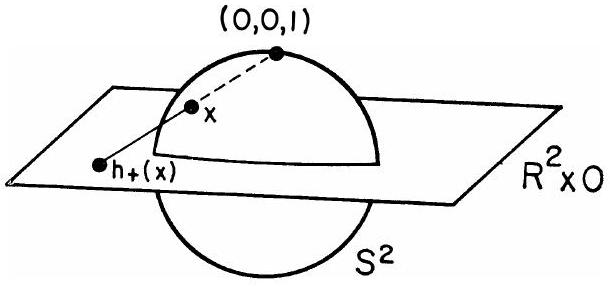
\includegraphics[scale=0.2, center]{2025_05_28_7c9927389b272ddbc2c3g-20}

Figure 3. Stereographic projection\\
hood of the north pole. To see this we introduce the stereographic projection $h_{-}$from the south pole $(0,0,-1)$ and set

$$
Q(z)=h_{-} f h_{-}^{-1}(z) .
$$

Note, by elementary geometry, that

$$
h_{+} h_{-}^{-1}(z)=z /|z|^{2}=1 / \bar{z} .
$$

Now if $P(z)=a_{0} z^{n}+a_{1} z^{n-1}+\cdots+a_{n}$, with $a_{0} \neq 0$, then a short computation shows that

$$
Q(z)=z^{n} /\left(\bar{a}_{0}+\bar{a}_{1} z+\cdots+\bar{a}_{n} z^{n}\right) .
$$

Thus $Q$ is smooth in a neighborhood of 0 , and it follows that $f=h_{-}^{-1} Q h_{-}$ is smooth in a neighborhood of $(0,0,1)$.

Next observe that $f$ has only a finite number of critical points; for $P$ fails to be a local diffeomorphism only at the zeros of the derivative polynomial $P^{\prime}(z)=\sum a_{n-i} j z^{j-1}$, and there are only finitely many zeros since $P^{\prime}$ is not identically zero. The set of regular values of $f$, being a sphere with finitely many points removed, is therefore connected. Hence the locally constant function $\# f^{-1}(y)$ must actually be constant on this set. Since $\# f^{-1}(y)$ can't be zero everywhere, we conclude that it is zero nowhere. Thus $f$ is an onto mapping, and the polynomial $P$ must have a zero.

\section*{§2. THE THEOREM OF SARD AND BROWN}
In general, it is too much to hope that the set of critical values of a smooth map be finite. But this set will be "small," in the sense indicated by the next theorem, which was proved by A. Sard in 1942 following earlier work by A. P. Morse. (References [30], [24].)

Theorem. 

\begin{THEO}{DT-M65-01-01}{Sard Theorem}
Let $f: U \rightarrow R^{n}$ be a smooth map, defined on an open set $U \subset R^{m}$, and let
$
C=\left\{x \varepsilon U \mid \quad \operatorname{rank} d f_{x}<n\right\} .
$
Then the image $f(C) \subset R^{n}$ has Lebesgue measure zero, i.e. given any $\epsilon>0$, it is possible to cover $f(C)$ by a sequence of cubes in $R^{n}$ having total $n$-dimensional volume less than $\epsilon$.

Since a set of measure zero cannot contain any nonvacuous open set, it follows that the complement $R^{n}-f(C)$ must be everywhere dense $\dagger$ in $R^{n}$.
\end{THEO}

The proof will be given in §3. It is essential for the proof that $f$ should have many derivatives. (Compare Whitney [38].)

We will be mainly interested in the case $m \geq n$. If $m<n$, then clearly $C=U$; hence the theorem says simply that $f(U)$ has measure zero.

More generally consider a smooth map $f: M \rightarrow N$, from a manifold of dimension $m$ to a manifold of dimension $n$. Let $C$ be the set of all $x \varepsilon M$ such that

$$
d f_{x}: T M_{x} \rightarrow T N_{f(x)}
$$


has rank less than $n$ (i.e. is not onto). Then $C$ will be called the set of critical points, $f(C)$ the set of critical values, and the complement $N-f(C)$ the set of regular values of $f$. (This agrees with our previous definitions in the case $m=n$.) Since $M$ can be covered by a countable collection of neighborhoods each diffeomorphic to an open subset of $R^{m}$, we have:

Corollary (A. B. Brown). 

\begin{KORO}{DT-M65-01-02}{Brown Korollar}
The set of regular values of a smooth map $f: M \rightarrow N$ is everywhere dense in $N$.
\end{KORO}

In order to exploit this corollary we will need the following:

Lemma 1. If $f: M \rightarrow N$ is a smooth map between manifolds of dimension $m \geq n$, and if $y \varepsilon N$ is a regular value, then the set $f^{-1}(y) \subset M$ is a smooth manifold of dimension $m-n$.

Proof. Let $x \varepsilon f^{-1}(y)$. Since $y$ is a regular value, the derivative $d f_{x}$ must map $T M_{x}$ onto $T N_{y}$. The null space $\mathfrak{N} \subset T M_{x}$ of $d f_{x}$ will therefore be an ( $m-n$ )-dimensional vector space.

If $M \subset R^{k}$, choose a linear map $L: R^{k} \rightarrow R^{m-n}$ that is nonsingular on this subspace $\Re \subset T M_{x} \subset R^{k}$. Now define

$$
F: M \rightarrow N \times R^{m-n}
$$

by $F(\xi)=(f(\xi), L(\xi))$. The derivative $d F_{x}$ is clearly given by the formula

$$
d F_{x}(v)=\left(d f_{x}(v), L(v)\right) .
$$

Thus $d F_{x}$ is nonsingular. Hence $F$ maps some neighborhood $U$ of $x$ diffeomorphically onto a neighborhood $V$ of ( $y, L(x)$ ). Note that $f^{-1}(y)$ corresponds, under $F$, to the hyperplane $y \times R^{m-n}$. In fact $F$ maps $f^{-1}(y) \cap U$ diffeomorphically onto $\left(y \times R^{m-n}\right) \cap V$. This proves that $f^{-1}(y)$ is a smooth manifold of dimension $m-n$.



As an example we can give an easy proof that the unit sphere $S^{m-1}$ is a smooth manifold. Consider the function $f: R^{m} \rightarrow R$ defined by

$$
f(x)=x_{1}^{2}+x_{2}^{2}+\cdots+x_{m}^{2}
$$

Any $y \neq 0$ is a regular value, and the smooth manifold $f^{-1}(1)$ is the unit sphere.

If $M^{\prime}$ is a manifold which is contained in $M$, it has already been noted that $T M_{x}^{\prime}$ is a subspace of $T M_{x}$ for $x \in M^{\prime}$. The orthogonal complement of $T M_{x}^{\prime}$ in $T M_{x}$ is then a vector space of dimension $m-m^{\prime}$ called the space of normal vectors to $M^{\prime}$ in $M$ at $x$.

In particular let $M^{\prime}=f^{-1}(y)$ for a regular value $y$ of $f: M \rightarrow N$.



Lemma 2. The null space of $d f_{x}: T M_{x} \rightarrow T N_{y}$ is precisely equal to the tangent space $T M_{x}^{\prime} \subset T M_{x}$ of the submanifold $M^{\prime}=f^{-1}(y)$. Hence $d f_{x}$ maps the orthogonal complement of $T M_{x}^{\prime}$ isomorphically onto $T N_{y}$.

Proof. From the diagram\\
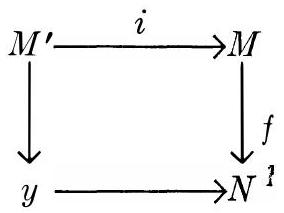
\includegraphics[scale=0.2, center]{2025_05_28_7c9927389b272ddbc2c3g-23}\\
we see that $d f_{x}$ maps the subspace $T M_{x}^{\prime} \subset T M_{x}$ to zero. Counting dimensions we see that $d f_{x}$ maps the space of normal vectors to $M^{\prime}$ isomorphically onto $T N_{\nu}$.


\pagebreak

\section*{MANIFOLDS WITH BOUNDARY}

The lemmas above can be sharpened so as to apply to a map defined on a smooth "manifold with boundary." Consider first the closed half-space
$$
H^{m}=\left\{\left(x_{1}, \cdots, x_{m}\right) \varepsilon R^{m} \mid x_{m} \geq 0\right\}
$$

The boundary $\partial H^{m}$ is defined to be the hyperplane $R^{m-1} \times 0 \subset R^{m}$.\\
Definition. A subset $X \subset R^{k}$ is called a smooth m-manifold with boundary if each $x \in X$ has a neighborhood $U \cap X$ diffeomorphic to an open subset $V \cap H^{m}$ of $H^{m}$. The boundary $\partial X$ is the set of all points in $X$ which correspond to points of $\partial H^{m}$ under such a diffeomorphism.

It is not hard to show that $\partial X$ is a well-defined smooth manifold of dimension $m-1$. The interior $X-\partial X$ is a smooth manifold of dimension $m$.

The tangent space $T X_{x}$ is defined just as in $\S 1$, so that $T X_{x}$ is a full $m$-dimensional vector space, even if $x$ is a boundary point.

Here is one method for generating examples. Let $M$ be a manifold without boundary and let $g: M \rightarrow R$ have 0 as regular value.



Lemma 3. The set of $x$ in $M$ with $g(x) \geq 0$ is a smooth manifold, with boundary equal to $g^{-1}(0)$.

The proof is just like the proof of Lemma 1.

Example. The unit disk $D^{m}$, consisting of all $x \in R^{m}$ with

$$
1-\sum x_{i}^{2} \geq 0
$$

is a smooth manifold, with boundary equal to $S^{m-1}$.\\
Now consider a smooth map $f: X \rightarrow N$ from an $m$-manifold with boundary to an $n$-manifold, where $m>n$.



Lemma 4. If $y \varepsilon N$ is a regular value, both for $f$ and for the restriction $f \mid \partial X$, then $f^{-1}(y) \subset X$ is a smooth ( $m-n$ )-manifold with boundary. Furthermore the boundary $\partial\left(f^{-1}(y)\right)$ is precisely equal to the intersection of $f^{-1}(y)$ with $\partial X$.

Proof. Since we have to prove a local property, it suffices to consider the special case of a map $f: H^{m} \rightarrow R^{n}$, with regular value $y \varepsilon R^{n}$. Let $\bar{x} \varepsilon f^{-1}(y)$. If $\bar{x}$ is an interior point, then as before $f^{-1}(y)$ is a smooth manifold in the neighborhood of $\bar{x}$.

Suppose that $\bar{x}$ is a boundary point. Choose a smooth map $g: U \rightarrow R^{n}$ that is defined throughout a neighborhood of $\bar{x}$ in $R^{m}$ and coincides with $f$ on $U \cap H^{m}$. Replacing $U$ by a smaller neighborhood if necessary, we may assume that $g$ has no critical points. Hence $g^{-1}(y)$ is a smooth manifold of dimension $m-n$.

Let $\pi: g^{-1}(y) \rightarrow R$ denote the coordinate projection,

$$
\pi\left(x_{1}, \cdots, x_{m}\right)=x_{m}
$$

We claim that $\pi$ has 0 as a regular value. For the tangent space of $g^{-1}(y)$ at a point $x \varepsilon \pi^{-1}(0)$ is equal to the null space of

$$
d g_{x}=d f_{x}: R^{m} \rightarrow R^{n} ;
$$

but the hypothesis that $f \mid \partial H^{m}$ is regular at $x$ guarantees that this null space cannot be completely contained in $R^{m-1} \times 0$.

Therefore the set $g^{-1}(y) \cap H^{m}=f^{-1}(y) \cap U$, consisting of all $x \varepsilon g^{-1}(y)$ with $\pi(x) \geq 0$, is a smooth manifold, by Lemma 3; with boundary equal to $\pi^{-1}(0)$. This completes the proof.

\section*{THE BROUWER FIXED POINT THEOREM}
We now apply this result to prove the key lemma leading to the classical Brouwer fixed point theorem. Let $X$ be a compact manifold with boundary.

Lemma 5. There is no smooth map $f: X \rightarrow \partial X$ that leaves $\partial X$ pointwise fixed.

Proof (following M. Hirsch). Suppose there were such a map $f$. Let $y \varepsilon \partial X$ be a regular value for $f$. Since $y$ is certainly a regular value for the identity map $f \mid \partial X$ also, it follows that $f^{-1}(y)$ is a smooth 1manifold, with boundary consisting of the single point

$$
f^{-1}(y) \cap \partial X=\{y\}
$$

But $f^{-1}(y)$ is also compact, and the only compact 1 -manifolds are finite disjoint unions of circles and segments,* so that $\partial f^{-1}(y)$ must consist of an even number of points. This contradiction establishes the lemma.

In particular the unit disk

$$
D^{n}=\left\{x \varepsilon R^{n} \mid x_{1}^{2}+\cdots+x_{n}^{2} \leq 1\right\}
$$

is a compact manifold bounded by the unit sphere $S^{n-1}$. Hence as a special case we have proved that the identity map of $S^{n-1}$ cannot be extended to a smooth map $D^{n} \rightarrow S^{n-1}$.

Lemma 6. Any smooth map $g: D^{n} \rightarrow D^{n}$ has a fixed point (i.e. a point $x \varepsilon D^{n}$ with $g(x)=x$ ).

Proof. Suppose $g$ has no fixed point. For $x \varepsilon D^{n}$, let $f(x) \varepsilon S^{n-1}$ be the point nearer $x$ on the line through $x$ and $g(x)$. (See Figure 4.) Then $f: D^{n} \rightarrow S^{n-1}$ is a smooth map with $f(x)=x$ for $x \varepsilon S^{n-1}$, which is impossible by Lemma 5. (To see that $f$ is smooth we make the following explicit computation: $f(x)=x+t u$, where

$$
u=\frac{x-g(x)}{\|x-g(x)\|}, \quad t=-x \cdot u+\sqrt{1-x \cdot x+(x \cdot u)^{2}}
$$

the expression under the square root sign being strictly positive. Here and subsequently $\|x\|$ denotes the euclidean length $\sqrt{x_{1}^{2}+\cdots+x_{n}^{2}}$.)

Brouwer Fixed Point Theorem. Any continuous function $G: D^{n} \rightarrow D^{n}$ has a fixed point.

Proof. We reduce this theorem to the lemma by approximating $G$ by a smooth mapping. Given $\epsilon>0$, according to the Weierstrass approximation theorem, $\dagger$ there is a polynomial function $P_{1}: R^{n} \rightarrow R^{n}$ with $\left\|P_{1}(x)-G(x)\right\|<\epsilon$ for $x \varepsilon D^{n}$. However, $P_{1}$ may send points

\footnotetext{\begin{itemize}
  \item A proof is given in the Appendix.\\
$\dagger$ See for example Dieudonné [7, p. 133].
\end{itemize}
}
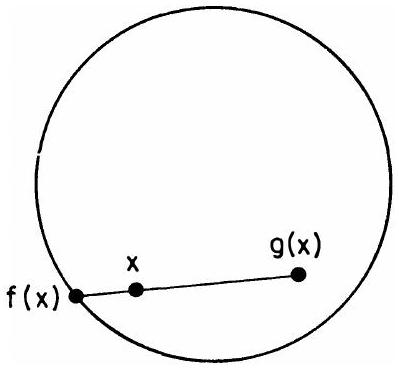
\includegraphics[scale=0.2, center]{2025_05_28_7c9927389b272ddbc2c3g-26}

Figure 4\\
of $D^{n}$ into points outside of $D^{n}$. To correct this we set

$$
P(x)=P_{1}(x) /(1+\epsilon) .
$$

Then clearly $P$ maps $D^{n}$ into $D^{n}$ and $\|P(x)-G(x)\|<2 \epsilon$ for $x \varepsilon D^{n}$.\\
Suppose that $G(x) \neq x$ for all $x \in D^{n}$. Then the continuous function $\|G(x)-x\|$ must take on a minimum $\mu>0$ on $D^{n}$. Choosing $P: D^{n} \rightarrow D^{n}$ as above, with $\|P(x)-G(x)\|<\mu$ for all $x$, we clearly have $P(x) \neq x$. Thus $P$ is a smooth map from $D^{n}$ to itself without a fixed point. This contradicts Lemma 6, and completes the proof.

The procedure employed here can frequently be applied in more general situations: to prove a proposition about continuous mappings, we first establish the result for smooth mappings and then try to use an approximation theorem to pass to the continuous case. (Compare §8, Problem 4.)

\section*{§3. PROOF OF SARD'S THEOREM*}
First let us recall the statement:\\
Theorem of Sard. Let $f: U \rightarrow R^{p}$ be a smooth map, with $U$ open in $R^{n}$, and let $C$ be the set of critical points; that is the set of all $x \in U$ with

$$
\operatorname{rank} d f_{x}<p
$$

Then $f(C) \subset R^{p}$ has measure zero.\\
Remark. The cases where $n \leq p$ are comparatively easy. (Compare de Rham [29, p. 10].) We will, however, give a unified proof which makes these cases look just as bad as the others.

The proof will be by induction on $n$. Note that the statement makes sense for $n \geq 0, p \geq 1$. (By definition $R^{0}$ consists of a single point.) To start the induction, the theorem is certainly true for $n=0$.

Let $C_{1} \subset C$ denote the set of all $x \quad \varepsilon U$ such that the first derivative $d f_{x}$ is zero. More generally let $C_{i}$ denote the set of $x$ such that all partial derivatives of $f$ of order $\leq i$ vanish at $x$. Thus we have a descending sequence of closed sets

$$
C \supset C_{1} \supset C_{2} \supset C_{3} \supset \cdots
$$

The proof will be divided into three steps as follows:\\
Step 1. The image $f\left(C-C_{1}\right)$ has measure zero.\\
Step 2. The image $f\left(C_{i}-C_{i+1}\right)$ has measure zero, for $i \geq 1$.\\
Step 3. The image $f\left(C_{k}\right)$ has measure zero for $k$ sufficiently large.\\
(Remark. If $f$ happens to be real analytic, then the intersection of

\footnotetext{\begin{itemize}
  \item Our proof is based on that given by Pontryagin [28]. The details are somewhat easier since we assume that $f$ is infinitely differentiable.
\end{itemize}
}
the $C_{i}$ is vacuous unless $f$ is constant on an entire component of $U$. Hence in this case it is sufficient to carry out Steps 1 and 2.)

Proof of Step 1. This first step is perhaps the hardest. We may assume that $p \geq 2$, since $C=C_{1}$ when $p=1$. We will need the well known theorem of Fubini* which asserts that a measurable set

$$
A \subset R^{p}=R^{1} \times R^{p-1}
$$

must have measure zero if it intersects each hyperplane (constant) $\times R^{p-1}$ in a set of ( $p-1$ )-dimensional measure zero.

For each $\bar{x} \varepsilon C-C_{1}$ we will find an open neighborhood $V \subset R^{n}$ so that $f(V \cap C)$ has measure zero. Since $C-C_{1}$ is covered by countably many of these neighborhoods, this will prove that $f\left(C-C_{1}\right)$ has measure zero.

Since $\bar{x} \notin C_{1}$, there is some partial derivative, say $\partial f_{1} / \partial x_{1}$, which is not zero at $\bar{x}$. Consider the map $h: U \rightarrow R^{n}$ defined by

$$
h(x)=\left(f_{1}(x), x_{2}, \cdots, x_{n}\right)
$$

Since $d h_{\tilde{x}}$ is nonsingular, $h$ maps some neighborhood $V$ of $\bar{x}$ diffeomorphically onto an open set $V^{\prime}$. The composition $g=f \circ h^{-1}$ will then map $V^{\prime}$ into $R^{p}$. Note that the set $C^{\prime}$ of critical points of $g$ is precisely $h(V \cap C)$; hence the set $g\left(C^{\prime}\right)$ of critical values of $g$ is equal to $f(V \cap C)$.\\
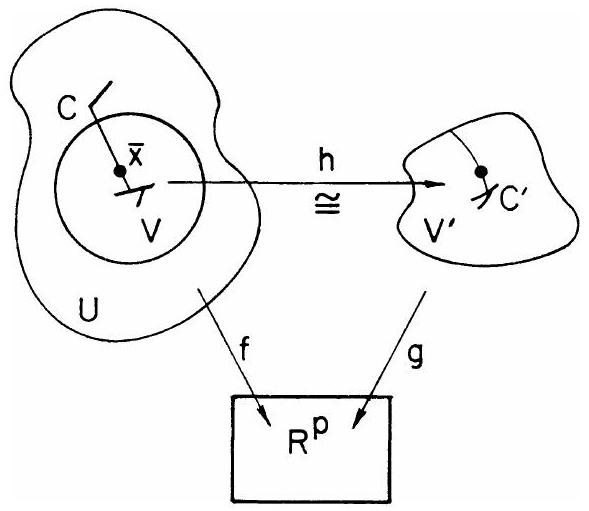
\includegraphics[scale=0.2, center]{2025_05_28_7c9927389b272ddbc2c3g-28}

Figure 5. Construction of the map $g$

\footnotetext{\begin{itemize}
  \item For an easy proof (as well as an alternative proof of Sard's theorem) see Sternberg [35, pp. 51-52]. Sternberg assumes that $A$ is compact, but the general case follows easily from this special case.
\end{itemize}
}For each $\left(t, x_{2}, \cdots, x_{n}\right) \varepsilon V^{\prime}$ note that $g\left(t, x_{2}, \cdots, x_{n}\right)$ belongs to the hyperplane $t \times R^{p-1} \subset R^{p}$ : thus $g$ carries hyperplanes into hyperplanes. Let

$$
g^{t}:\left(t \times R^{n-1}\right) \cap V^{\prime} \rightarrow t \times R^{p-1}
$$

denote the restriction of $g$. Note that a point of $t \times R^{n-1}$ is critical for $g^{t}$ if and only if it is critical for $g$; for the matrix of first derivatives of $g$ has the form

$$
\left(\partial g_{i} / \partial x_{j}\right)=\left(\begin{array}{cc}
1 & 0 \\
* & \left(\partial g_{i}^{t} / \partial x_{j}\right)
\end{array}\right)
$$

According to the induction hypothesis, the set of critical values of $g^{t}$ has measure zero in $t \times R^{p-1}$. Therefore the set of critical values of $g$ intersects each hyperplane $t \times R^{p-1}$ in a set of measure zero. This set $g\left(C^{\prime}\right)$ is measurable, since it can be expressed as a countable union of compact subsets. Hence, by Fubini's theorem, the set

$$
g\left(C^{\prime}\right)=f(V \cap C)
$$

has measure zero, and Step 1 is complete.\\
Proof of Step 2. For each $\bar{x} \varepsilon C_{k}-C_{k+1}$ there is some $(k+1)^{-s t}$ derivative $\partial^{k+1} f_{r} / \partial x_{s_{1}} \ldots \partial x_{s_{k+1}}$ which is not zero. Thus the function

$$
w(x)=\partial^{k} f_{r} / \partial x_{s_{2}} \cdots \partial x_{s_{k+1}}
$$

vanishes at $\bar{x}$ but $\partial w / \partial x_{s_{1}}$ does not. Suppose for definiteness that $s_{1}=1$. Then the map $h: U \rightarrow R^{n}$ defined by

$$
h(x)=\left(w(x), x_{2}, \cdots, x_{n}\right)
$$

carries some neighborhood $V$ of $\bar{x}$ diffeomorphically onto an open set $V^{\prime}$. Note that $h$ carries $C_{k} \cap V$ into the hyperplane $0 \times R^{n-1}$. Again we consider

$$
g=f \circ h^{-1}: V^{\prime} \rightarrow R^{p}
$$

Let

$$
\bar{g}:\left(0 \times R^{n-1}\right) \cap V^{\prime} \rightarrow R^{p}
$$

denote the restriction of $g$. By induction, the set of critical values of $\bar{g}$ has measure zero in $R^{p}$. But each point in $h\left(C_{k} \cap V\right)$ is certainly a critical point of $\bar{g}$ (since all derivatives of order $\leq k$ vanish). Therefore

$$
\bar{g} h\left(C_{k} \cap V\right)=f\left(C_{k} \cap V\right) \text { has measure zero. }
$$

Since $C_{k}-C_{k+1}$ is covered by countably many such sets $V$, it follows that $f\left(C_{k}-C_{k+1}\right)$ has measure zero.

Proof of Step 3. Let $I^{n} \subset U$ be a cube with edge $\delta$. If $k$ is sufficiently large ( $k>n / p-1$ to be precise) we will prove that $f\left(C_{k} \cap I^{n}\right)$ has measure zero. Since $C_{k}$ can be covered by countably many such cubes, this will prove that $f\left(C_{k}\right)$ has measure zero.

From Taylor's theorem, the compactness of $I^{n}$, and the definition of $C_{k}$, we see that

$$
f(x+h)=f(x)+R(x, h)
$$

where

$$
\|R(x, h)\| \leq c\|h\|^{k+1}
$$

for $x \varepsilon C_{k} \cap I^{n}, x+h \varepsilon I^{n}$. Here $c$ is a constant which depends only on $f$ and $I^{n}$. Now subdivide $I^{n}$ into $r^{n}$ cubes of edge $\delta / r$. Let $I_{1}$ be a cube of the subdivision which contains a point $x$ of $C_{k}$. Then any point of $I_{1}$ can be written as $x+h$, with

$$
\|h\| \leq \sqrt{n}(\delta / r)
$$

From 1) it follows that $f\left(I_{1}\right)$ lies in a cube of edge $a / r^{k+1}$ centered about $f(x)$, where $a=2 c(\sqrt{n} \delta)^{k+1}$ is constant. Hence $f\left(C_{k} \cap I^{n}\right)$ is contained in a union of at most $r^{n}$ cubes having total volume

$$
V \leq r^{n}\left(a / r^{k+1}\right)^{p}=a^{p} r^{n-(k+1) p}
$$

If $k+1>n / p$, then evidently $V$ tends to 0 as $r \rightarrow \infty$; so $f\left(C_{k} \cap I^{n}\right)$ must have measure zero. This completes the proof of Sard's theorem.

\section*{§4. THE DEGREE MODULO 2 OF A MAPPING}
Consider a smooth map $f: S^{n} \rightarrow S^{n}$. If $y$ is a regular value, recall that $\# f^{-1}(y)$ denotes the number of solutions $x$ to the equation $f(x)=y$. We will prove that the residue class modulo 2 of $\# f^{-1}(y)$ does not depend on the choice of the regular value $y$. This residue class is called the mod 2 degree of $f$. More generally this same definition works for any smooth map

$$
f: M \rightarrow N
$$

where $M$ is compact without boundary, $N$ is connected, and both manifolds have the same dimension. (We may as well assume also that $N$ is compact without boundary, since otherwise the mod 2 degree would necessarily be zero.) For the proof we introduce two new concepts.

\section*{SMOOTH HOMOTOPY AND SMOOTH ISOTOPY}
Given $X \subset R^{k}$, let $X \times[0,1]$ denote the subset* of $R^{k+1}$ consisting of all ( $x, t$ ) with $x \in X$ and $0 \leq t \leq 1$. Two mappings

$$
f, g: X \rightarrow Y
$$

are called smoothly homotopic (abbreviated $f \sim g$ ) if there exists a

\footnotetext{\begin{itemize}
  \item If $M$ is a smooth manifold without boundary, then $M \times[0,1]$ is a smooth manifold bounded by two "copies" of $M$. Boundary points of $M$ will give rise to "corner" points of $M \times[0,1]$.
\end{itemize}
}
smooth map $F: X \times[0,1] \rightarrow Y$ with
$$
F(x, 0)=f(x), \quad F(x, 1)=g(x)
$$
for all $x \in X$. This map $F$ is called a smooth homotopy between $f$ and $g$.\\
Note that the relation of smooth homotopy is an equivalence relation. To see that it is transitive we use the existence of a smooth function $\varphi:[0,1] \rightarrow[0,1]$ with\\


\[
\begin{aligned}
& \varphi(t)=0 \quad \text { for } \quad 0 \leq t \leq \frac{1}{3} \\
& \varphi(t)=1 \quad \text { for } \quad \frac{2}{3} \leq t \leq 1 .
\end{aligned}
\]


(For example, let $\varphi(t)=\lambda\left(t-\frac{1}{3}\right) /\left(\lambda\left(t-\frac{1}{3}\right)+\lambda\left(\frac{2}{3}-t\right)\right)$, where $\lambda(\tau)=0$ for $\tau \leq 0$ and $\lambda(\tau)=\exp \left(-\tau^{-1}\right)$ for $\tau>0$.) Given a smooth homotopy $F$ between $f$ and $g$, the formula $G(x, t)=F(x, \varphi(t))$ defines a smooth homotopy $G$ with


\[
\begin{aligned}
& G(x, t)=f(x) \quad \text { for } \quad 0 \leq t \leq \frac{1}{3} \\
& G(x, t)=g(x) \quad \text { for } \quad \frac{2}{3} \leq t \leq 1
\end{aligned}
\]

Now if $f \sim g$ and $g \sim h$, then, with the aid of this construction, it is easy to prove that $f \sim h$.

If $f$ and $g$ happen to be diffeomorphisms from $X$ to $Y$, we can also define the concept of a "smooth isotopy" between $f$ and $g$. This also will be an equivalence relation.

Definition. The diffeomorphism $f$ is smoothly isotopic to $g$ if there exists a smooth homotopy $F: X \times[0,1] \rightarrow Y$ from $f$ to $g$ so that, for each $t \varepsilon[0,1]$, the correspondence

$$
x \rightarrow F(x, t)
$$

maps $X$ diffeomorphically onto $Y$.\\
It will turn out that the mod 2 degree of a map depends only on its smooth homotopy class:

Homotopy Lemma. Let $f, g: M \rightarrow N$ be smoothly homotopic maps between manifolds of the same dimension, where $M$ is compact and without boundary. If $y \varepsilon N$ is a regular value for both $f$ and $g$, then

$$
\# f^{-1}(y) \equiv \# g^{-1}(y) \quad(\bmod 2) .
$$

Proof. Let $F: M \times[0,1] \rightarrow N$ be a smooth homotopy between $f$ and $g$. First suppose that $y$ is also a regular value for $F$. Then $F^{-1}(y)$\\
is a compact 1-manifold, with boundary equal to

$$
F^{-1}(y) \cap(M \times 0 \cup M \times 1)=f^{-1}(y) \times 0 \cup g^{-1}(y) \times 1 .
$$

Thus the total number of boundary points of $F^{-1}(y)$ is equal to

$$
\# f^{-1}(y)+\# g^{-1}(y) .
$$

But we recall from §2 that a compact 1-manifold always has an even number of boundary points. Thus $\# f^{-1}(y)+\# g^{-1}(y)$ is even, and therefore

$$
\# f^{-1}(y) \equiv \# g^{-1}(y) \quad(\bmod 2) .
$$

\begin{center}
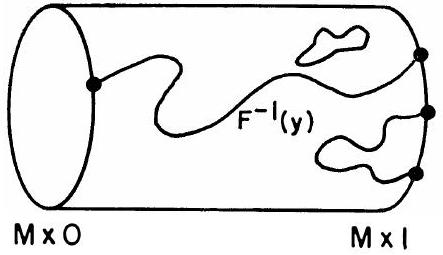
\includegraphics[scale=0.2]{2025_05_28_7c9927389b272ddbc2c3g-33}
\end{center}

Figure 6. The number of boundary points on the left is congruent to the number on the right modulo 2

Now suppose that $y$ is not a regular value of $F$. Recall (from §1) that $\# f^{-1}\left(y^{\prime}\right)$ and $\# g^{-1}\left(y^{\prime}\right)$ are locally constant functions of $y^{\prime}$ (as long as we stay away from critical values). Thus there is a neighborhood $V_{1} \subset N$ of $y$, consisting of regular values of $f$, so that

$$
\# f^{-1}\left(y^{\prime}\right)=\# f^{-1}(y)
$$

for all $y^{\prime} \varepsilon V_{1}$; and there is an analogous neighborhood $V_{2} \subset N$ so that

$$
\# g^{-1}\left(y^{\prime}\right)=\# g^{-1}(y)
$$

for all $y^{\prime} \varepsilon V_{2}$. Choose a regular value $z$ of $F$ within $V_{1} \cap V_{2}$. Then

$$
\left.\# f^{-1}(y)=\# f^{-1}(z) \equiv \# g^{-1}(z)=\# g^{-1}(y)\right),
$$

which completes the proof.\\
We will also need the following:\\
Homogeneity Lemma. Let $y$ and $z$ be arbitrary interior points of the smooth, connected man ifold $N$. Then there exists a diffeomorphism $h: N \rightarrow N$ that is smoothly isotopic to the identity and carries $y$ into $z$.\\
(For the special case $N=S^{n}$ the proof is easy: simply choose $h$ to be the rotation which carries $y$ into $z$ and leaves fixed all vectors orthogonal to the plane through $y$ and $z$.)

The proof in general proceeds as follows: We will first construct a smooth isotopy from $R^{n}$ to itself which

\begin{enumerate}
  \item leaves all points outside of the unit ball fixed, and
  \item slides the origin to any desired point of the open unit ball.\\
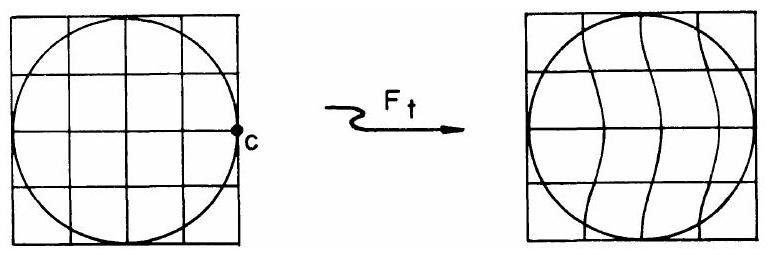
\includegraphics[scale=0.2, center]{2025_05_28_7c9927389b272ddbc2c3g-34}
\end{enumerate}

Figure 7. Deforming the unit ball

Let $\varphi: R^{n} \rightarrow R$ be a smooth function which satisfies

$$
\begin{array}{ll}
\varphi(x)>0 & \text { for } \quad\|x\|<1 \\
\varphi(x)=0 & \text { for } \quad\|x\| \geq 1
\end{array}
$$

(For example let $\varphi(x)=\lambda\left(1-\|x\|^{2}\right)$ where $\lambda(t)=0$ for $t \leq 0$ and $\lambda(t)=\exp \left(-t^{-1}\right)$ for $t>0$.) Given any fixed unit vector $c \varepsilon S^{n-1}$, consider the differential equations

$$
\frac{\mathrm{d} x_{i}}{\mathrm{~d} t}=c_{i} \varphi\left(x_{1}, \cdots, x_{n}\right) ; \quad i=1, \cdots, n .
$$

For any $\bar{x} \varepsilon R^{n}$ these equations have a unique solution $x=x(t)$, defined for all* real numbers which satisfies the initial condition

$$
x(0)=\bar{x} .
$$

We will use the notation $x(t)=F_{t}(\bar{x})$ for this solution. Then clearly

\begin{enumerate}
  \item $F_{t}(\bar{x})$ is defined for all $t$ and $\bar{x}$ and depends smoothly on $t$ and $\bar{x}$,
  \item $F_{0}(\bar{x})=\bar{x}$,
  \item $F_{s+t}(\bar{x})=F_{s} \circ F_{t}(\bar{x})$.
\end{enumerate}

\footnotetext{\begin{itemize}
  \item Compare [22, §2.4].
\end{itemize}
}Therefore each $F_{t}$ is a diffeomorphism from $R^{n}$ onto itself. Letting $t$ vary, we see that each $F_{t}$ is smoothly isotopic to the identity under an isotopy which leaves all points outside of the unit ball fixed. But clearly, with suitable choice of $c$ and $t$, the diffeomorphism $F_{t}$ will carry the origin to any desired point in the open unit ball.

Now consider a connected manifold $N$. Call two points of $N$ "isotopic" if there exists a smooth isotopy carrying one to the other. This is clearly an equivalence relation. If $y$ is an interior point, then it has a neighborhood diffeomorphic to $R^{n}$; hence the above argument shows that every point sufficiently close to $y$ is "isotopic" to $y$. In other words, each "isotopy class" of points in the interior of $N$ is an open set, and the interior of $N$ is partitioned into disjoint open isotopy classes. But the interior of $N$ is connected; hence there can be only one such isotopy class. This completes the proof.

We can now prove the main result of this section. Assume that $M$ is compact and boundaryless, that $N$ is connected, and that $f: M \rightarrow N$ is smooth.

Theorem. If $y$ and $z$ are regular values of $f$ then

$$
\# f^{-1}(y) \equiv \# f^{-1}(z) \quad(\text { modulo } 2) .
$$

This common residue class, which is called the mod 2 degree of $f$, depends only on the smooth homotopy class of $f$.

Proof. Given regular values $y$ and $z$, let $h$ be a diffeomorphism from $N$ to $N$ which is isotopic to the identity and which carries $y$ to $z$. Then $z$ is a regular value of the composition $h \circ f$. Since $h \circ f$ is homotopic to $f$, the Homotopy Lemma asserts that

$$
\#(h \circ f)^{-1}(z) \equiv \# f^{-1}(z) \quad(\bmod 2) .
$$

But

$$
(h \circ f)^{-1}(z)=f^{-1} h^{-1}(z)=f^{-1}(y)
$$

so that

$$
\#(h \circ f)^{-1}(z)=\# f^{-1}(y) .
$$

Therefore

$$
\# f^{-1}(y) \equiv \# f^{-1}(z) \quad(\bmod 2),
$$

as required.\\
Call this common residue class $\operatorname{deg}_{2}(f)$. Now suppose that $f$ is smoothly homotopic to $g$. By Sard's theorem, there exists an element $y \varepsilon N$\\
which is a regular value for both $f$ and $g$. The congruence

$$
\operatorname{deg}_{2} f \equiv \# f^{-1}(y) \equiv \# g^{-1}(y) \equiv \operatorname{deg}_{2} g
$$

now shows that $\operatorname{deg}_{2} f$ is a smooth homotopy invariant, and completes the proof.

Examples. A constant map $c: M \rightarrow M$ has even mod 2 degree. The identity map $I$ of $M$ has odd degree. Hence the identity map of a compact boundaryless manifold is not homotopic to a constant.

In the case $M=S^{n}$, this result implies the assertion that no smooth map $f: D^{n+1} \rightarrow S^{n}$ leaves the sphere pointwise fixed. (I.e., the sphere is not a smooth "retract" of the disk. Compare §2, Lemma 5.) For such a map $f$ would give rise to a smooth homotopy

$$
F: S^{n} \times[0,1] \rightarrow S^{n}, \quad F(x, t)=f(t x)
$$

between a constant map and the identity.

\section*{§5. ORIENTED MANIFOLDS}
In order to define the degree as an integer (rather than an integer modulo 2) we must introduce orientations.

Definitions. An orientation for a finite dimensional real vector space is an equivalence class of ordered bases as follows: the ordered basis ( $b_{1}, \cdots, b_{n}$ ) determines the same orientation as the basis ( $b_{1}^{\prime}, \cdots, b_{n}^{\prime}$ ) if $b_{i}^{\prime}=\sum a_{i j} b_{j}$ with $\operatorname{det}\left(a_{i j}\right)>0$. It determines the opposite orientation if $\operatorname{det}\left(a_{i j}\right)<0$. Thus each positive dimensional vector space has precisely two orientations. The vector space $R^{n}$ has a standard orientation corresponding to the basis $(1,0, \cdots, 0),(0,1,0, \cdots, 0), \cdots,(0, \cdots, 0,1)$.

In the case of the zero dimensional vector space it is convenient to define an "orientation" as the symbol +1 or -1 .

An oriented smooth manifold consists of a manifold $M$ together with a choice of orientation for each tangent space $T M_{x}$. If $m \geq 1$, these are required to fit together as follows: For each point of $M$ there should exist a neighborhood $U \subset M$ and a diffeomorphism $h$ mapping $U$ onto an open subset of $R^{m}$ or $H^{m}$ which is orientation preserving, in the sense that for each $x \in U$ the isomorphism $d h_{x}$ carries the specified orientation for $T M_{x}$ into the standard orientation for $R^{m}$.

If $M$ is connected and orientable, then it has precisely two orientations.

If $M$ has a boundary, we can distinguish three kinds of vectors in the tangent space $T M_{x}$ at a boundary point:

\begin{enumerate}
  \item there are the vectors tangent to the boundary, forming an ( $m-1$ )dimensional subspace $T(\partial M)_{x} \subset T M_{x}$;
  \item there are the "outward" vectors, forming an open half space bounded by $T(\partial M)_{x}$;
  \item there are the "inward" vectors forming a complementary half space.
\end{enumerate}

Each orientation for $M$ determines an orientation for $\partial M$ as follows: For $x \varepsilon \partial M$ choose a positively oriented basis $\left(v_{1}, v_{2}, \cdots, v_{m}\right)$ for $T M_{x}$ in such a way that $v_{2}, \cdots, v_{m}$ are tangent to the boundary (assuming that $m \geq 2$ ) and that $v_{1}$ is an "outward" vector. Then ( $v_{2}, \cdots, v_{m}$ ) determines the required orientation for $\partial M$ at $x$.

If the dimension of $M$ is 1 , then each boundary point $x$ is assigned the orientation -1 or +1 according as a positively oriented vector at $x$ points inward or outward. (See Figure 8.)\\
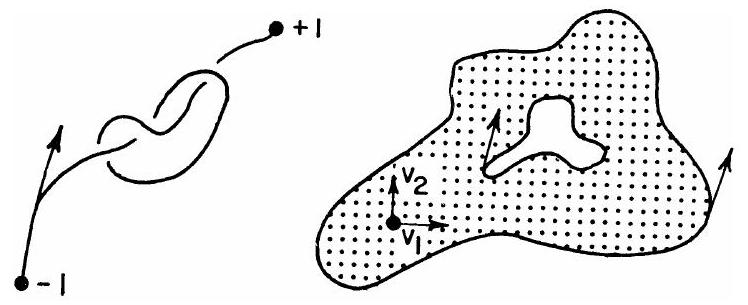
\includegraphics[scale=0.2, center]{2025_05_28_7c9927389b272ddbc2c3g-38}

Figure 8. How to orient a boundary

As an example the unit sphere $S^{m-1} \subset R^{m}$ can be oriented as the boundary of the disk $D^{m}$.

\section*{THE BROUWER DEGREE}
Now let $M$ and $N$ be oriented $n$-dimensional manifolds without boundary and let

$$
f: M \rightarrow N
$$

be a smooth map. If $M$ is compact and $N$ is connected, then the degree of $f$ is defined as follows:

Let $x \in M$ be a regular point of $f$, so that $d f_{x}: T M_{x} \rightarrow T N_{f(x)}$ is a linear isomorphism between oriented vector spaces. Define the sign of $d f_{x}$ to be +1 or -1 according as $d f_{x}$ preserves or reverses orientation. For any regular value $y \varepsilon N$ define

$$
\operatorname{deg}(f ; y)=\sum_{x \varepsilon f^{-1}(y)} \operatorname{sign} d f_{x}
$$

As in §1, this integer $\operatorname{deg}(f ; y)$ is a locally constant function of $y$. It is defined on a dense open subset of $N$.

Theorem A. The integer $\operatorname{deg}(f ; y)$ does not depend on the choice of regular value $y$.

It will be called the degree of $f$ (denoted $\operatorname{deg} f$ ).\\
Theorem B. If $f$ is smoothiy homotopic to $g$, then $\operatorname{deg} f=\operatorname{deg} g$.\\
The proof will be essentially the same as that in §4. It is only necessary to keep careful control of orientations.

First consider the following situation: Suppose that $M$ is the boundary of a compact oriented manifold $X$ and that $M$ is oriented as the boundary of $X$.

Lemma 1. If $f: M \rightarrow N$ extends to a smooth map $F: X \rightarrow N$, then $\operatorname{deg}(f ; y)=0$ for every regular value $y$.

Proof. First suppose that $y$ is a regular value for $F$, as well as for $f=F \mid M$. The compact 1-manifold $F^{-1}(y)$ is a finite union of arcs and circles, with only the boundary points of the arcs lying on $M=\partial X$. Let $A \subset F^{-1}(y)$ be one of these arcs, with $\partial A=\{a\} \cup\{b\}$. We will show that

$$
\operatorname{sign} d f_{a}+\operatorname{sign} d f_{b}=0
$$

and hence (summing over all such arcs) that $\operatorname{deg}(f ; y)=0$.\\
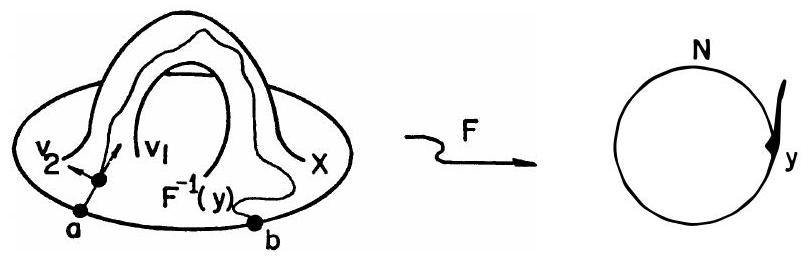
\includegraphics[scale=0.2, center]{2025_05_28_7c9927389b272ddbc2c3g-39}

Figure 9. How to orient $F^{-1}(y)$

The orientations for $X$ and $N$ determine an orientation for $A$ as follows: Given $x \in A$, let $\left(v_{1}, \cdots, v_{n+1}\right)$ be a positively oriented basis for $T X_{x}$ with $v_{1}$ tangent to $A$. Then $v_{1}$ determines the required orientation for $T A_{x}$ if and only if $d F_{x}$ carries $\left(v_{2}, \cdots, v_{n+1}\right)$ into a positively oriented basis for $T N_{y}$.

Let $v_{1}(x)$ denote the positively oriented unit vector tangent to $A$ at $x$. Clearly $v_{1}$ is a smooth function, and $v_{1}(x)$ points outward at one boundary point (say $b$ ) and inward at the other boundary point $a$.

It follows immediately that

$$
\operatorname{sign} d f_{a}=-1, \quad \operatorname{sign} d f_{b}=+1 ;
$$

with sum zero. Adding up over all such arcs $A$, we have proved that $\operatorname{deg}(f ; y)=0$.

More generally, suppose that $y_{0}$ is a regular value for $f$, but not for $F$. The function $\operatorname{deg}(f ; y)$ is constant within some neighborhood $U$ of $y_{0}$. Hence, as in §4, we can choose a regular value $y$ for $F$ within $U$ and observe that

$$
\operatorname{deg}\left(f ; y_{0}\right)=\operatorname{deg}(f ; y)=0 .
$$

This proves Lemma 1.\\
Now consider a smooth homotopy $\quad F:[0,1] \times M \rightarrow N \quad$ between two mappings $\quad f(x)=F(0, x), \quad g(x)=F(1, x)$.

Lemma 2. The degree $\operatorname{deg}(g ; y)$ is equal to $\operatorname{deg}(f ; y)$ for any common regular value $y$.

Proof. The manifold $[0,1] \times M^{n}$ can be oriented as a product, and will then have boundary consisting of $1 \times M^{n}$ (with the correct orientation) and $0 \times M^{n}$ (with the wrong orientation). Thus the degree of $F \mid \partial\left([0,1] \times M^{n}\right)$ at a regular value $y$ is equal to the difference

$$
\operatorname{deg}(g ; y)-\operatorname{deg}(f ; y)
$$

According to Lemma 1 this difference must be zero.\\
The remainder of the proof of Theorems A and B is completely analogous to the argument in §4. If $y$ and $z$ are both regular values for $f: M \rightarrow N$, choose a diffeomorphism $h: N \rightarrow N$ that carries $y$ to $z$ and is isotopic to the identity. Then $h$ will preserve orientation, and

$$
\operatorname{deg}(f ; y)=\operatorname{deg}(h \circ f ; h(y))
$$

by inspection. But $f$ is homotopic to $h \circ f$; hence

$$
\operatorname{deg}(h \circ f ; z)=\operatorname{deg}(f ; z)
$$

by Lemma 2. Therefore $\operatorname{deg}(f ; y)=\operatorname{deg}(f ; z)$, which completes the proof.\\
Examples. The complex function $z \rightarrow z^{k}, z \neq 0$, maps the unit circle onto itself with degree $k$. (Here $k$ may be positive, negative, or zero.) The degenerate mapping

$$
f: M \rightarrow \text { constant } \varepsilon N
$$

has degree zero. A diffeomorphism $f: M \rightarrow N$ has degree +1 or -1 according as $f$ preserves or reverses orientation. Thus an orientation reversing diffeomorphism of a compact boundaryless manifold is not smoothly homotopic to the identity.

One example of an orientation reversing diffeomorphism is provided by the reflection $r_{i}: S^{n} \rightarrow S^{n}$, where

$$
r_{\imath}\left(x_{1}, \cdots, x_{n+1}\right)=\left(x_{1}, \cdots,-x_{i}, \cdots, x_{n+1}\right) .
$$

The antipodal map of $S^{n}$ has degree $(-1)^{n+1}$, as we can see by noting that the antipodal map is the composition of $n+1$ reflections:

$$
-x=r_{1} \circ r_{2} \circ \cdots \circ r_{n+1}(x) .
$$

Thus if $n$ is even, the antipodal map of $S^{n}$ is not smoothly homotopic to the identity, a fact not detected by the degree modulo 2 .

As an application, following Brouwer, we show that $S^{n}$ admits a smooth field of nonzero tangent vectors if and only if $n$ is odd. (Compare Figures 10 and 11.)\\
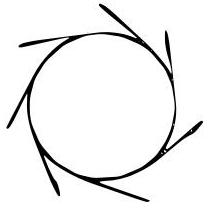
\includegraphics[scale=0.2, center]{2025_05_28_7c9927389b272ddbc2c3g-41(1)}

Figure 10 (above). A nonzero vector field on the 1-sphere

Figure 11 (below). Attempts for $n=2$\\
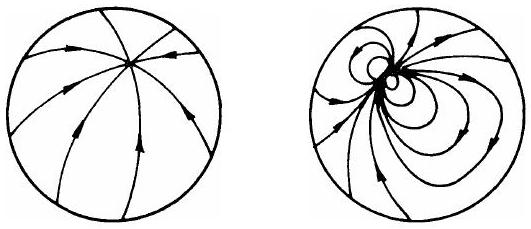
\includegraphics[scale=0.2, center]{2025_05_28_7c9927389b272ddbc2c3g-41}

Definition. A smooth tangent vector field on $M \subset R^{k}$ is a smooth map $v: M \rightarrow R^{k}$ such that $v(x) \varepsilon T M_{x}$ for each $x \varepsilon M$. In the case of the sphere $S^{n} \subset R^{n+1}$ this is clearly equivalent to the condition

$$
v(x) \cdot x=0 \quad \text { for all } \quad x \varepsilon S^{n},
$$

using the euclidean inner product.\\
If $v(x)$ is nonzero for all $x$, then we may as well suppose that

$$
v(x) \cdot v(x)=1 \quad \text { for all } \quad x \varepsilon S^{n} .
$$

For in any case $\bar{v}(x)=v(x) /\|v(x)\|$ would be a vector field which does satisfy this condition. Thus we can think of $v$ as a smooth function from $S^{n}$ to itself.

Now define a smooth homotopy

$$
F: S^{n} \times[0, \pi] \rightarrow S^{n}
$$

by the formula $F(x, \theta)=x \cos \theta+v(x) \sin \theta$. Computation shows that

$$
F(x, \theta) \cdot F(x, \theta)=1
$$

and that

$$
F(x, 0)=x, \quad F(x, \pi)=-x .
$$

Thus the antipodal map of $S^{n}$ is homotopic to the identity. But for $n$ even we have seen that this is impossible.

On the other hand, if $n=2 k-1$, the explicit formula

$$
v\left(x_{1}, \cdots, x_{2 k}\right)=\left(x_{2},-x_{1}, x_{4},-x_{3}, \cdots, x_{2 k},-x_{2 k-1}\right)
$$

defines a nonzero tangent vector field on $S^{n}$. This completes the proof.\\
It follows, incidentally, that the antipodal map of $S^{n}$ is homotopic to the identity for $n$ odd. A famous theorem due to Heinz Hopf asserts that two mappings from a connected $n$-manifold to the $n$-sphere are smoothly homotopic if and only if they have the same degree. In §7 we will prove a more general result which implies Hopf's theorem.

\section*{§6. VECTOR FIELDS AND THE EULER NUMBER}
As a further application of the concept of degree, we study vector fields on other manifolds.

Consider first an open set $U \subset R^{m}$ and a smooth vector field

$$
v: U \rightarrow R^{m}
$$

with an isolated zero at the point $z \varepsilon U$. The function

$$
\bar{v}(x)=v(x) /\|v(x)\|
$$

maps a small sphere centered at $z$ into the unit sphere.* The degree of this mapping is called the index $\iota$ of $v$ at the zero $z$.

Some examples, with indices $-1,0,1,2$, are illustrated in Figure 12. (Intimately associated with $v$ are the curves "tangent" to $v$ which are obtained by solving the differential equations $\mathrm{d} x_{i} / \mathrm{d} t=v_{i}\left(x_{1}, \cdots, x_{n}\right)$. It is these curves which are actually sketched in Figure 12.)

A zero with arbitrary index can be obtained as follows: In the plane of complex numbers the polynomial $z^{k}$ defines a smooth vector field with a zero of index $k$ at the origin, and the function $\bar{z}^{k}$ defines a vector field with a zero of index -k .

We must prove that this concept of index is invariant under diffeomorphism of $U$. To explain what this means, let us consider the more general situation of a map $f: M \rightarrow N$, with a vector field on each manifold.

Definition. The vector fields $v$ on $M$ and $v^{\prime}$ on $N$ correspond under $f$ if the derivative $d f_{x}$ carries $v(x)$ into $v^{\prime}(f(x))$ for each $x \in M$.

\footnotetext{\begin{itemize}
  \item Each sphere is to be oriented as the boundary of the corresponding disk.
\end{itemize}
}
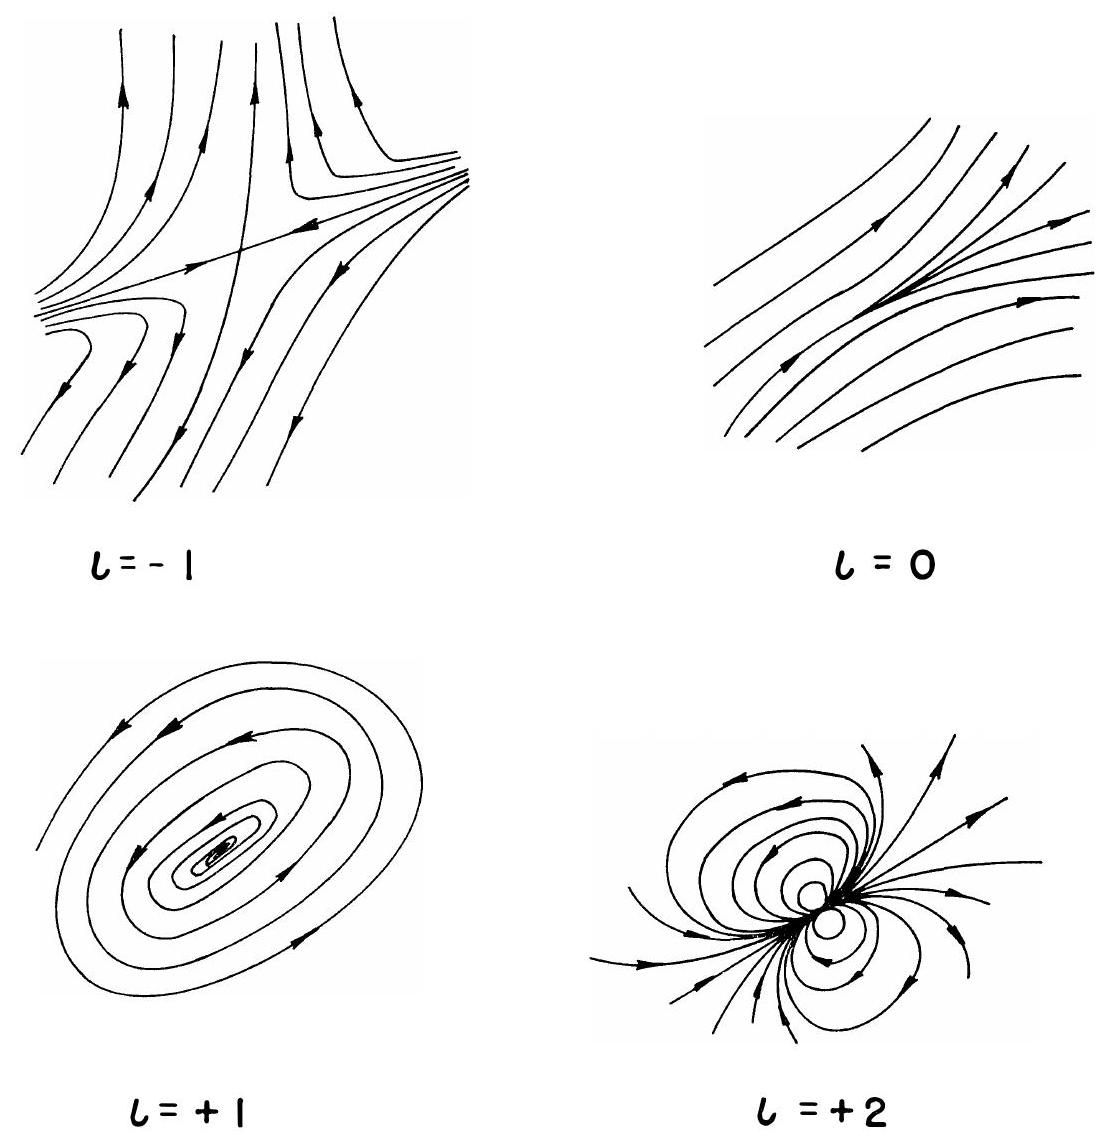
\includegraphics[scale=0.2, center]{2025_05_28_7c9927389b272ddbc2c3g-44}

Figure 12. Examples of plane vector fields

If $f$ is a diffeomorphism, then clearly $v^{\prime}$ is uniquely determined by $v$. The notation

$$
v^{\prime}=d f \circ v \circ f^{-1}
$$

will be used.\\
Lemma 1. Suppose that the vector field $v$ on $U$ corresponds to

$$
v^{\prime}=d f \circ v \circ f^{-1}
$$

on $U^{\prime}$ under a diffeomorphism $f: U \rightarrow U^{\prime}$. Then the index of $v$ at an isolated zero $z$ is equal to the index of $v^{\prime}$ at $f(z)$.

Assuming Lemma 1, we can define the concept of index for a vector field $w$ on an arbitrary manifold $M$ as follows: If $g: U \rightarrow M$ is a parametrization of a neighborhood of $z$ in $M$, then the index $\iota$ of $w$ at $z$ is defined to be equal to the index of the corresponding vector field $d g^{-1} \circ w \circ g$ on $U$ at the zero $g^{-1}(z)$. It clearly will follow from Lemma 1 that $\iota$ is well defined.

The proof of Lemma 1 will be based on the proof of a quite different result:

Lemma 2. Any orientation preserving diffeomorphism $f$ of $R^{m}$ is smoothly isotopic to the identity.\\
(In contrast, for many values of $m$ there exists an orientation preserving diffeomorphism of the sphere $S^{m}$ which is not smoothly isotopic to the identity. See [20, p. 404].)

Proof. We may assume that $f(0)=0$. Since the derivative at 0 can be defined by

$$
d f_{0}(x)=\lim _{t \rightarrow 0} f(t x) / t,
$$

it is natural to define an isotopy

$$
F: R^{m} \times[0,1] \rightarrow R^{m}
$$

by the formula

$$
\begin{aligned}
& F(x, t)=f(t x) / t \quad \text { for } \quad 0<t \leq 1, \\
& F(x, 0)=d f_{0}(x) .
\end{aligned}
$$

To prove that $F$ is smooth, even as $t \rightarrow 0$, we write $f$ in the form*

$$
f(x)=x_{1} g_{1}(x)+\cdots+x_{m} g_{m}(x),
$$

where $g_{1}, \cdots, g_{m}$ are suitable smooth functions, and note that

$$
F(x, t)=x_{1} g_{1}(t x)+\cdots+x_{m} g_{m}(t x)
$$

for all values of $t$.\\
Thus $f$ is isotopic to the linear mapping $d f_{0}$, which is clearly isotopic to the identity. This proves Lemma 2.

Proof of Lemma 1. We may assume that $z=f(z)=0$ and that $U$ is convex. If $f$ preserves orientation, then, proceeding exactly as above,

\footnotetext{\begin{itemize}
  \item See for example [22, p. 5].
\end{itemize}
}
we construct a one-parameter family of embeddings
$$
f_{t}: U \rightarrow R^{m}
$$
with $f_{0}=$ identity, $f_{1}=f$, and $f_{t}(0)=0$ for all $t$. Let $v_{t}$ denote the vector field $d f_{t} \circ v \circ f_{t}^{-1}$ on $f_{t}(U)$, which corresponds to $v$ on $U$. These vector fields are all defined and nonzero on a sufficiently small sphere centered at 0 . Hence the index of $v=v_{0}$ at 0 must be equal to the index of $v^{\prime}=v_{1}$ at 0 . This proves Lemma 1 for orientation preserving diffeomorphisms.

To consider diffeomorphisms which reverse orientation it is sufficient to consider the special case of a reflection $\rho$. Then

$$
v^{\prime}=\rho \circ v \circ \rho^{-1}
$$

so the associated function $\bar{v}^{\prime}(x)=v^{\prime}(x) /\left\|v^{\prime}(x)\right\|$ on the $\epsilon$-sphere satisfies

$$
\bar{v}^{\prime}=\rho \circ \bar{v} \circ \rho^{-1} .
$$

Evidently the degree of $\bar{v}^{\prime}$ equals the degree of $\bar{v}$, which completes the proof of Lemma 1.

We will study the following classical result: Let $M$ be a compact manifold and $w$ a smooth vector field on $M$ with isolated zeros. If $M$ has a boundary, then $w$ is required to point outward at all boundary points.

Poincaré-Hopf Theorem. The sum $\sum_{\iota}$ of the indices at the zeros of such a vector field is equal to the Euler number*

$$
\chi(M)=\sum_{i=0}^{m}(-1)^{i} \quad \mathrm{rank} \quad H_{i}(M)
$$

In particular this index sum is a topological invariant of $M$ : it does not depend on the particular choice of vector field.\\[0pt]
(A 2-dimensional version of this theorem was proved by Poincaré in 1885. The full theorem was proved by Hopf [14] in 1926 after earlier partial results by Brouwer and Hadamard.)

We will prove part of this theorem, and sketch a proof of the rest. First consider the special case of a compact domain in $R^{m}$.

Let $X \subset R^{m}$ be a compact $m$-manifold with boundary. The Gauss mapping

$$
g: \partial X \rightarrow S^{m-1}
$$

assigns to each $x \varepsilon \partial X$ the outward unit normal vector at $x$.

\footnotetext{\begin{itemize}
  \item Here $H_{i}(M)$ denotes the $i$-th homology group of $M$. This will be our first and last reference to homology theory.
\end{itemize}
}Lemma 3 (Hopf). If $v: X \rightarrow R^{m}$ is a smooth vector field with isolated zeros, and if $v$ points out of $X$ along the boundary, then the index sum $\sum$ c is equal to the degree of the Gauss mapping from $\partial X$ to $S^{m-1}$. In particular, $\sum$ i does not depend on the choice of $v$.

For example, if a vector field on the disk $D^{m}$ points outward along the boundary, then $\sum \iota=+1$. (Compare Figure 13.)\\
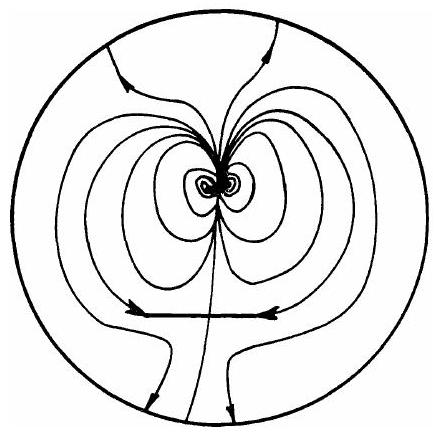
\includegraphics[scale=0.2, center]{2025_05_28_7c9927389b272ddbc2c3g-47}

Figure 13. An example with index sum +1

Proof. Removing an $\epsilon$-ball around each zero, we obtain a new manifold with boundary. The function $\bar{v}(x)=v(x) /\|v(x)\|$ maps this manifold into $S^{m-1}$. Hence the sum of the degrees of $\bar{v}$ restricted to the various boundary components is zero. But $\bar{v} \mid \partial X$ is homotopic to $g$, and the degrees on the other boundary components add up to $-\sum \iota$. (The minus sign occurs since each small sphere gets the wrong orientation.) Therefore

$$
\operatorname{deg}(g)-\sum \iota=0
$$

as required.\\
Remark. The degree of $g$ is also known as the "curvatura integra" of $\partial X$, since it can be expressed as a constant times the integral over $\partial X$ of the Gaussian curvature. This integer is of course equal to the Euler number of $X$. For $m$ odd it is equal to half the Euler number of $\partial X$.

Before extending this result to other manifolds, some more preliminaries are needed.

It is natural to try to compute the index of a vector field $v$ at a zero $z$\\
in terms of the derivatives of $v$ at $z$. Consider first a vector field $v$ on an open set $U \subset R^{m}$ and think of $v$ as a mapping $U \rightarrow R^{m}$, so that $d v_{z}: R^{m} \rightarrow R^{m}$ is defined.

Definition. The vector field $v$ is nondegenerate at $z$ if the linear transformation $d v_{z}$ is nonsingular.

It follows that $z$ is an isolated zero.\\
Lemma 4. The index of $v$ at a nondegenerate zero $z$ is either +1 or -1 according as the determinant of $d v_{z}$ is positive or negative.

Proof. Think of $v$ as a diffeomorphism from some convex neighborhood $U_{0}$ of $z$ into $R^{m}$. We may assume that $z=0$. If $v$ preserves orientation, we have seen that $v \mid U_{0}$ can be deformed smoothly into the identity without introducing any new zeros. (See Lemmas 1, 2.) Hence the index is certainly equal to +1 .

If $v$ reverses orientation, then similarly $v$ can be deformed into a reflection; hence $\iota=-1$.

More generally consider a zero $z$ of a vector field $w$ on a manifold $M \subset R^{k}$. Think of $w$ as a map from $M$ to $R^{k}$ so that the derivative $d w_{z}: T M_{z} \rightarrow R^{k}$ is defined.

Lemma 5. The derivative $d w_{z}$ actually carries $T M_{z}$ into the subspace $T M_{z} \subset R^{k}$, and hence can be considered as a linear transformation from $T M_{z}$ to itself. If this linear transformation has determinant $D \neq 0$ then $z$ is an isolated zero of $w$ with index equal to +1 or -1 according as $D$ is positive or negative.

Proof. Let $h: U \rightarrow M$ be a parametrization of some neighborhood of $z$. Let $e^{i}$ denote the $i$-th basis vector of $R^{m}$ and let

$$
t^{i}=d h_{u}\left(e^{i}\right)=\partial h / \partial u_{i}
$$

so that the vectors $t^{1}, \cdots, t^{m}$ form a basis for the tangent space $T M_{h(u)}$. We must compute the image of $t^{i}=t^{i}(u)$ under the linear transformation $d w_{h(u)}$. First note that

$$
d w_{h(u)}\left(t^{i}\right)=d(w \circ h)_{u}\left(e^{i}\right)=\partial w(h(u)) / \partial u_{i} .
$$

Let $v=\sum v_{i} e^{i}$ be the vector field on $U$ which corresponds to the vector field $w$ on $M$. By definition $v=d h^{-1} \circ w \circ h$, so that

$$
w(h(u))=d h_{u}(v)=\sum v_{i} t^{i}
$$

Therefore

$$
\partial w(h(u)) / \partial u_{i}=\sum_{i}\left(\partial v_{i} / \partial u_{i}\right) t^{i}+\sum_{i} v_{i}\left(\partial t^{i} / \partial u_{i}\right) .
$$

Combining 1) and 2), and then evaluating at the zero $h^{-1}(z)$ of $v$, we obtain the formula

$$
d w_{z}\left(t^{i}\right)=\sum_{j}\left(\partial v_{j} / \partial u_{i}\right) t^{j} .
$$

Thus $d w_{z}$ maps $T M_{z}$ into itself, and the determinant $D$ of this linear transformation $T M_{z} \rightarrow T M_{z}$ is equal to the determinant of the matrix $\left(\partial v_{i} / \partial u_{i}\right)$. Together with Lemma 4 this completes the proof.

Now consider a compact, boundaryless manifold $M \subset R^{k}$. Let $N_{\epsilon}$ denote the closed $\epsilon$-neighborhood of $M$ (i.e., the set of all $x \in R^{k}$ with $\|x-y\| \leq \epsilon$ for some $y \varepsilon M$ ). For $\epsilon$ sufficiently small one can show that $N_{\epsilon}$ is a smooth manifold with boundary. (See §8, Problem 11.)

Theorem 1. For any vector field $v$ on $M$ with only nondegenerate zeros, the index sum $\sum$ is equal to the degree of the Gauss mapping*

$$
g: \partial N_{\epsilon} \rightarrow S^{k-1} .
$$

In particular this sum does not depend on the choice of vector field.\\
Proof. For $x \in N_{\epsilon}$ let $r(x) \in M$ denote the closest point of $M$. (Compare §8, Problem 12.) Note that the vector $x-r(x)$ is perpendicular to the tangent space of $M$ at $r(x)$, for otherwise $r(x)$ would not be the closest point of $M$. If $\epsilon$ is sufficiently small, then the function $r(x)$ is smooth and well defined.\\
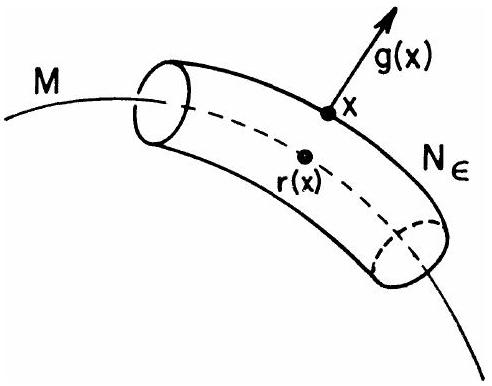
\includegraphics[scale=0.2, center]{2025_05_28_7c9927389b272ddbc2c3g-49}

Figure 14. The $\epsilon$-neighborhood of $M$

\footnotetext{\begin{itemize}
  \item A different interpretation of this degree has been given by Allendoerfer and Fenchel: the degree of $g$ can be expressed as the integral over $M$ of a suitable curvature scalar, thus yielding an $m$-dimensional version of the classical Gauss-Bonnet theorem. (References [1], [9]. See also Chern [6].)
\end{itemize}
}We will also consider the squared distance function

$$
\varphi(x)=\|x-r(x)\|^{2} .
$$

An easy computation shows that the gradient of $\varphi$ is given by

$$
\operatorname{grad} \varphi=2(x-r(x))
$$

Hence, for each point $x$ of the level surface $\partial N_{\epsilon}=\varphi^{-1}\left(\epsilon^{2}\right)$, the outward unit normal vector is given by

$$
g(x)=\operatorname{grad} \varphi /\|\operatorname{grad} \varphi\|=(x-r(x)) / \epsilon .
$$

Extend $v$ to a vector field $w$ on the neighborhood $N_{\epsilon}$ by setting

$$
w(x)=(x-r(x))+v(r(x))
$$

Then $w$ points outward along the boundary, since the inner product $w(x) \cdot g(x)$ is equal to $\epsilon>0$. Note that $w$ can vanish only at the zeros of $v$ in $M$; this is clear since the two summands $(x-r(x))$ and $v(r(x))$ are mutually orthogonal. Computing the derivative of $w$ at a zero $z \varepsilon M$, we see that

$$
\begin{array}{ll}
d w_{z}(h)=d v_{z}(h) & \text { for all } h \varepsilon T M_{z} \\
d w_{z}(h)=h & \text { for } h \varepsilon T M_{z}^{\perp}
\end{array}
$$

Thus the determinant of $d w_{z}$ is equal to the determinant of $d v_{z}$. Hence the index of $w$ at the zero $z$ is equal to the index $\iota$ of $v$ at $z$.

Now according to Lemma 3 the index sum $\sum \iota$ is equal to the degree of $g$. This proves Theorem 1.

Examples. On the sphere $S^{m}$ there exists a vector field $v$ which points "north" at every point.* At the south pole the vectors radiate outward; hence the index is +1 . At the north pole the vectors converge inward; hence the index is $(-1)^{m}$. Thus the invariant $\sum \iota$ is equal to 0 or 2 according as $m$ is odd or even. This gives a new proof that every vector field on an even sphere has a zero.

For any odd-dimensional, boundaryless manifold the invariant $\sum \iota$ is zero. For if the vector field $v$ is replaced by $-v$, then each index is multiplied by $(-1)^{m}$, and the equality

$$
\sum \iota=(-1)^{m} \sum \iota
$$

for $m$ odd, implies that $\sum \iota=0$.

\footnotetext{\begin{itemize}
  \item For example, $v$ can be defined by the formula $v(x)=p-(p \cdot x) x$, where $p$ is the north pole. (See Figure 11.)
\end{itemize}
}Remark. If $\sum \iota=0$ on a connected manifold $M$, then a theorem of Hopf asserts that there exists a vector field on $M$ with no zeros at all.

In order to obtain the full strength of the Poincaré-Hopf theorem, three further steps are needed.

Step 1. Identification of the invariant $\sum$ i with the Euler number $\chi(M)$. It is sufficient to construct just one example of a nondegenerate vector field on $M$ with $\sum \iota$ equal to $\chi(M)$. The most pleasant way of doing this is the following: According to Marston Morse, it is always possible to find a real valued function on $M$ whose "gradient" is a nondegenerate vector field. Furthermore, Morse showed that the sum of indices associated with such a gradient field is equal to the Euler number of $M$. For details of this argument the reader is referred to Milnor [22, pp. 29, 36].

Step 2. Proving the theorem for a vector field with degenerate zeros. Consider first a vector field $v$ on an open set $U$ with an isolated zero at $z$. If

$$
\lambda: U \rightarrow[0,1]
$$

takes the value 1 on a small neighborhood $N_{1}$ of $z$ and the value 0 outside a slightly larger neighborhood $N$, and if $y$ is a sufficiently small regular value of $v$, then the vector field

$$
v^{\prime}(x)=v(x)-\lambda(x) y
$$

is nondegenerate* within $N$. The sum of the indices at the zeros within $N$ can be evaluated as the degree of the map

$$
\bar{v}: \partial N \rightarrow S^{m-1}
$$

and hence does not change during this alteration.\\
More generally consider vector fields on a compact manifold $M$. Applying this argument locally we see that any vector field with isolated zeros can be replaced by a nondegenerate vector field without altering the integer $\sum \iota$.

Step 3. Manifolds with boundary. If $M \subset R^{k}$ has a boundary, then any vector field $v$ which points outward along $\partial M$ can again be extended over the neighborhood $N_{\epsilon}$ so as to point outward along $\partial N_{\epsilon}$. However, there is some difficulty with smoothness around the boundary of $M$. Thus $N_{\epsilon}$ is not a smooth (i.e. differentiable of class $C^{\infty}$ ) manifold,

\footnotetext{\begin{itemize}
  \item Clearly $v^{\prime}$ is nondegenerate within $N_{1}$. But if $y$ is sufficiently small, then $v^{\prime}$ will have no zeros at all within $N-N_{1}$.
\end{itemize}
}
but only a $C^{1}$-manifold. The extension $w$, if defined as before by $w(x)=v(r(x))+x-r(x)$, will only be a continuous vector field near $\partial M$. The argument can nonetheless be carried out either by showing that our strong differentiability assumptions are not really necessary or by other methods.

\section*{§7. FRAMED COBORDISM THE PONTRYAGIN CONSTRUCTION}
The degree of a mapping $M \rightarrow M^{\prime}$ is defined only when the manifolds $M$ and $M^{\prime}$ are oriented and have the same dimension. We will study a generalization, due to Pontryagin, which is defined for a smooth map

$$
f: M \rightarrow S^{p}
$$

from an arbitrary compact, boundaryless manifold to a sphere. First some definitions.

Let $N$ and $N^{\prime}$ be compact $n$-dimensional submanifolds of $M$ with $\partial N=\partial N^{\prime}=\partial M=\varnothing$. The difference of dimensions $m-n$ is called the codimension of the submanifolds.

Definition. $N$ is cobordant to $N^{\prime}$ within $M$ if the subset

$$
N \times[0, \epsilon) \cup N^{\prime} \times(1-\epsilon, 1]
$$

of $M \times[0,1]$ can be extended to a compact manifold

$$
X \subset M \times[0,1]
$$

so that

$$
\partial X=N \times 0 \cup N^{\prime} \times 1,
$$

and so that $X$ does not intersect $M \times 0 \cup M \times 1$ except at the points of $\partial X$.

Clearly cobordism is an equivalence relation. (See Figure 15.)\\
Definition. A framing of the submanifold $N \subset M$ is a smooth function $\mathfrak{v}$ which assigns to each $x \in N$ a basis

$$
\mathfrak{b}(x)=\left(v^{1}(x), \cdots, v^{m-n}(x)\right)
$$

for the space $T N_{x}^{\perp} \subset T M_{x}$ of normal vectors to $N$ in $M$ at $x$. (See\\
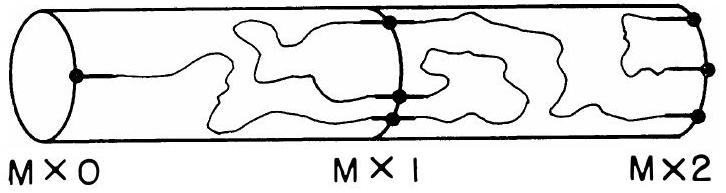
\includegraphics[scale=0.2, center]{2025_05_28_7c9927389b272ddbc2c3g-54}

Figure 15. Pasting together two cobordisms within $M$

Figure 16.) The pair ( $N, \mathfrak{b}$ ) is called a framed submanifold of $M$. Two framed submanifolds ( $N, \mathfrak{b}$ ) and ( $N^{\prime}, \mathfrak{w}$ ) are framed cobordant if there exists a cobordism $X \subset M \times[0,1]$ between $N$ and $N^{\prime}$ and a framing $\mathfrak{u}$ of $X$, so that

$$
\begin{array}{cll}
u^{i}(x, t)=\left(v^{i}(x), 0\right) & \text { for } & (x, t) \varepsilon N \times[0, \epsilon) \\
u^{i}(x, t)=\left(w^{i}(x), 0\right) & \text { for } & (x, t) \varepsilon N^{\prime} \times(1-\epsilon, 1] .
\end{array}
$$

Again this is an equivalence relation.\\
Now consider a smooth map $f: M \rightarrow S^{p}$ and a regular value $y \varepsilon S^{p}$. The map $f$ induces a framing of the manifold $f^{-1}(y)$ as follows: Choose a positively oriented basis $\mathfrak{v}=\left(v^{1}, \cdots, v^{p}\right)$ for the tangent space $T\left(S^{p}\right)_{y}$. For each $x \varepsilon f^{-1}(y)$ recall from page 12 that

$$
d f_{x}: T M_{x} \rightarrow T\left(S^{p}\right)_{y}
$$

maps the subspace $T f^{-1}(y)_{x}$ to zero and maps its orthogonal complement $T f^{-1}(y)_{x}^{\perp}$ isomorphically onto $T\left(S^{p}\right)_{y}$. Hence there is a unique vector

$$
w^{i}(x) \varepsilon T f^{-1}(y)_{x}^{\perp} \subset T M_{x}
$$

that maps into $v^{i}$ under $d f_{x}$. It will be convenient to use the notation $\mathfrak{w}=f^{*} \mathfrak{y}$ for the resulting framing $w^{1}(x), \cdots, w^{p}(x)$ of $f^{-1}(y)$.

Definition. This framed manifold ( $f^{-1}(y), f^{*} \mathfrak{b}$ ) will be called the Pontryagin manifold associated with $f$.

Of course $f$ has many Pontryagin manifolds, corresponding to different choices of $y$ and $\mathfrak{v}$, but they all belong to a single framed cobordism class:

Theorem A. If $y^{\prime}$ is another regular value of $f$ and $\mathfrak{v}^{\prime}$ is a positively oriented basis for $T\left(S^{p}\right)_{y^{\prime}}$, then the framed manifold $\left(f^{-1}\left(y^{\prime}\right), f^{*} \mathfrak{v}^{\prime}\right)$ is framed cobordant to ( $f^{-1}(y), f^{*} \mathfrak{b}$ ).

Theorem B. Two mappings from $M$ to $S^{p}$ are smoothly homotopic if and only if the associated Pontryagin manifolds are framed cobordant.\\
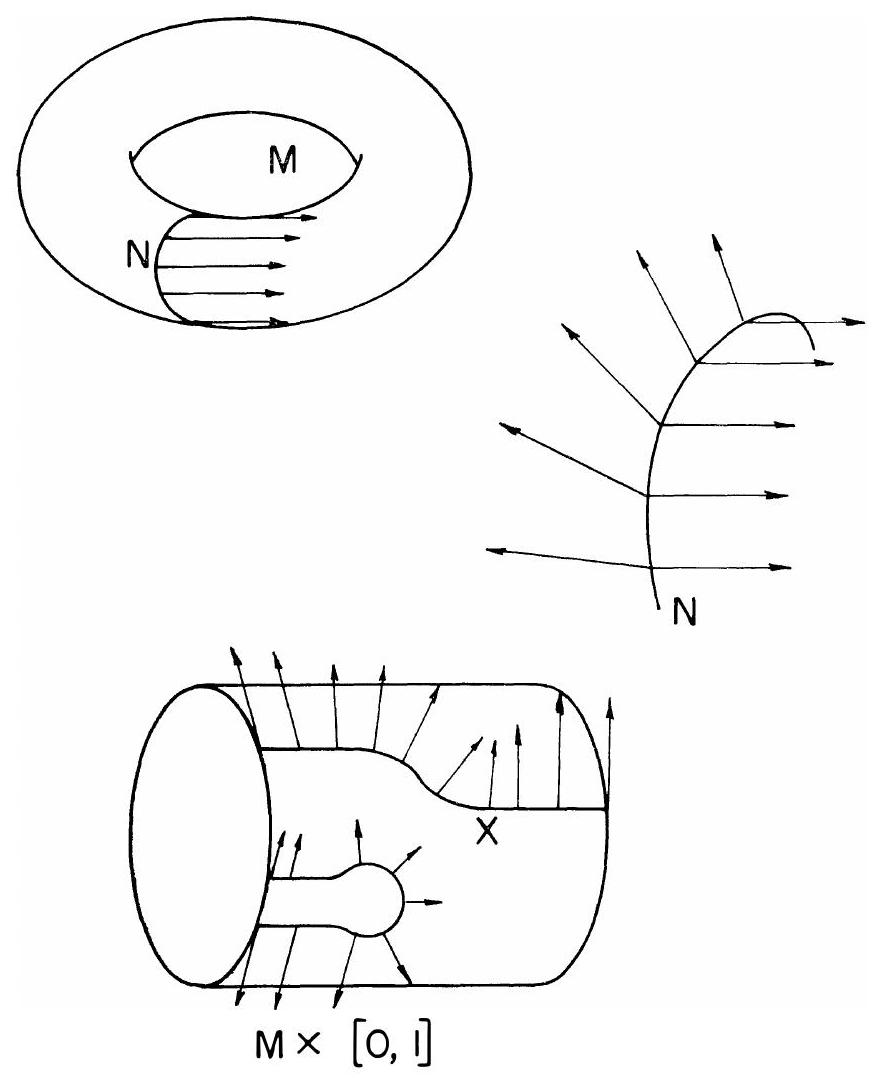
\includegraphics[scale=0.2, center]{2025_05_28_7c9927389b272ddbc2c3g-55}

Figure 16. Framed submanifolds and a framed cobordism

Theorem C. Any compact framed submanifold ( $N, \mathfrak{w}$ ) of codimension $p$ in $M$ occurs as Pontryagin manifold for some smooth mapping $f: M \rightarrow S^{p}$.

Thus the homotopy classes of maps are in one-one correspondence with the framed cobordism classes of submanifolds.

The proof of Theorem A will be very similar to the arguments in $\S \S 4$ and 5. It will be based on three lemmas.

Lemma 1. If $\mathfrak{b}$ and $\mathfrak{v}^{\prime}$ are two different positively oriented bases at $y$, then the Pontryagin manifold ( $f^{-1}(y), f^{*} \mathfrak{b}$ ) is framed cobordant to ( $f^{-1}(y)$, $\left.f^{*} \mathfrak{v}^{\prime}\right)$.

Proof. Choose a smooth path from $\mathfrak{v}$ to $\mathfrak{v}^{\prime}$ in the space of all positively oriented bases for $T\left(S^{p}\right)_{y}$. This is possible since this space of bases\\
can be identified with the space $G L^{+}(p, R)$ of matrices with positive determinant, and hence is connected. Such a path gives rise to the required framing of the cobordism $f^{-1}(y) \times[0,1]$.

By abuse of notation we will often delete reference to $f^{*} \mathfrak{v}$ and speak simply of "the framed manifold $f^{-1}(y)$."

Lemma 2. If $y$ is a regular value of $f$, and $z$ is sufficiently close to $y$, then $f^{-1}(z)$ is framed cobordant to $f^{-1}(y)$.

Proof. Since the set $f(C)$ of critical values is compact, we can choose $\epsilon>0$ so that the $\epsilon$-neighborhood of $y$ contains only regular values. Given $z$ with $\|z-y\|<\epsilon$, choose a smooth one-parameter family of rotations (i.e. an isotopy) $r_{t}: S^{p} \rightarrow S^{p}$ so that $r_{1}(y)=z$, and so that

\begin{enumerate}
  \item $r_{t}$ is the identity for $0 \leq t<\epsilon^{\prime}$,
  \item $r_{t}$ equals $r_{1}$ for $1-\epsilon^{\prime}<t \leq 1$, and
  \item each $r_{t}^{-1}(z)$ lies on the great circle from $y$ to $z$, and hence is a regular value of $f$.
\end{enumerate}

Define the homotopy

$$
F: M \times[0,1] \rightarrow S^{p}
$$

by $F(x, t)=r_{t} f(x)$. For each $t$ note that $z$ is a regular value of the composition

$$
r_{\iota} \circ f: M \rightarrow S^{p} .
$$

It follows a fortiori that $z$ is a regular value for the mapping $F$. Hence

$$
F^{-1}(z) \subset M \times[0,1]
$$

is a framed manifold and provides a framed cobordism between the framed manifolds $f^{-1}(z)$ and $\left(r_{1} \circ f\right)^{-1}(z)=f^{-1} r_{1}^{-1}(z)=f^{-1}(y)$. This proves Lemma 2.

Lemma 3. If $f$ and $g$ are smoothly homotopic and $y$ is a regular value for both, then $f^{-1}(y)$ is framed cobordant to $g^{-1}(y)$.

Proof. Choose a homotopy $F$ with

$$
\begin{array}{ll}
F(x, t)=f(x) & 0 \leq t<\epsilon, \\
F(x, t)=g(x) & 1-\epsilon<t \leq 1 .
\end{array}
$$

Choose a regular value $z$ for $F$ which is close enough to $y$ so that $f^{-1}(z)$ is framed cobordant to $f^{-1}(y)$ and so that $g^{-1}(z)$ is framed cobordant to $g^{-1}(y)$. Then $F^{-1}(z)$ is a framed manifold and provides a framed cobordism between $f^{-1}(z)$ and $g^{-1}(z)$. This proves Lemma 3.

Proof of Theorem A. Given any two regular values $y$ and $z$ for $f$, we can choose rotations

$$
r_{t}: S^{p} \rightarrow S^{p}
$$

so that $r_{0}$ is the identity and $r_{1}(y)=z$. Thus $f$ is homotopic to $r_{1} \circ f$; hence $f^{-1}(z)$ is framed cobordant to

$$
\left(r_{1} \circ f\right)^{-1}(z)=f^{-1} r_{1}^{-1}(z)=f^{-1}(y) .
$$

This completes the proof of Theorem A.\\
The proof of Theorem C will be based on the following: Let $N \subset M$ be a framed submanifold of codimension $p$ with framing $\mathfrak{v}$. Assume that $N$ is compact and that $\partial N=\partial M=\varnothing$.

Product Neighborhood Theorem. Some neighborhood of $N$ in $M$ is diffeomorphic to the product $N \times R^{p}$. Furthermore the diffeomorphism can be chosen so that each $x \in N$ corresponds to $(x, 0) \in N \times R^{p}$ and so that each normal frame $\mathfrak{v}(x)$ corresponds to the standard basis for $R^{p}$.

Remark. Product neighborhoods do not exist for arbitrary submanifolds. (Compare Figure 17.)\\
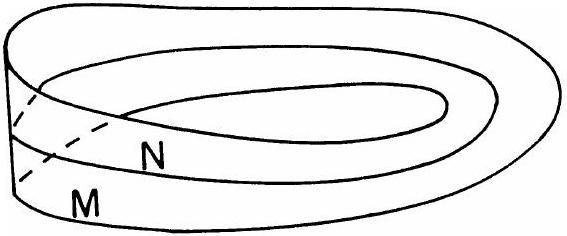
\includegraphics[scale=0.2, center]{2025_05_28_7c9927389b272ddbc2c3g-57}

Figure 17. An unframable submanifold

Proof. First suppose that $M$ is the euclidean space $R^{n+p}$. Consider the mapping $g: N \times R^{p} \rightarrow M$, defined by

$$
g\left(x ; t_{1}, \cdots, t_{p}\right)=x+t_{1} v^{1}(x)+\cdots+t_{p} v^{p}(x) .
$$

Clearly $d g_{(x ; 0, \cdots, 0)}$ is nonsingular; hence $g$ maps some neighborhood of ( $x, 0$ ) $\varepsilon N \times R^{p}$ diffeomorphically onto an open set.

We will prove that $g$ is one-one on the entire neighborhood $N \times U_{\epsilon}$ of $N \times 0$, providing that $\epsilon>0$ is sufficiently small; where $U_{\epsilon}$ denotes the $\epsilon$-neighborhood of 0 in $R^{p}$. For otherwise there would exist pairs $(x, u) \neq\left(x^{\prime}, u^{\prime}\right)$ in $N \times R^{p}$ with $\|u\|$ and $\left\|u^{\prime}\right\|$ arbitrarily small and with

$$
g(x, u)=g\left(x^{\prime}, u^{\prime}\right) .
$$

Since $N$ is compact, we could choose a sequence of such pairs with $x$ converging, say to $x_{0}$, with $x^{\prime}$ converging to $x_{0}^{\prime}$, and with $u \rightarrow 0$ and $u^{\prime} \rightarrow 0$. Then clearly $x_{0}=x_{0}^{\prime}$, and we have contradicted the statement that $g$ is one-one in a neighborhood of ( $x_{0}, 0$ ).

Thus $g$ maps $N \times U_{\epsilon}$ diffeomorphically onto an open set. But $U_{\epsilon}$ is diffeomorphic to the full euclidean space $R^{p}$ under the correspondence

$$
u \rightarrow u /\left(1-\|u\|^{2} / \epsilon^{2}\right) .
$$

Since $g(x, 0)=x$, and since $d g_{(x, 0)}$ does what is expected of it, this proves the Product Neighborhood Theorem for the special case $M=R^{n+p}$.

For the general case it is necessary to replace straight lines in $R^{n+p}$ by geodesics in $M$. More precisely let $g\left(x ; t_{1}, \cdots, t_{p}\right)$ be the endpoint of the geodesic segment of length $\left\|t_{1} v^{1}(x)+\cdots+t_{p} v^{p}(x)\right\|$ in $M$ which starts at $x$ with the initial velocity vector

$$
t_{1} v^{1}(x)+\cdots+t_{p} v^{p}(x) /\left\|t_{1} v^{1}(x)+\cdots+t_{p} v^{p}(x)\right\|
$$

The reader who is familiar with geodesics will have no difficulty in checking that

$$
g: N \times U_{\epsilon} \rightarrow M
$$

is well defined and smooth, for $\epsilon$ sufficiently small. The remainder of the proof proceeds exactly as before.

Proof of Theorem C. Let $N \subset M$ be a compact, boundaryless, framed submanifold. Choose a product representation

$$
g: N \times R^{p} \rightarrow V \subset M
$$

for a neighborhood $V$ of $N$, as above, and define the projection

$$
\pi: V \rightarrow R^{p}
$$

by $\pi(g(x, y))=y$. (See Figure 18.) Clearly 0 is a regular value, and $\pi^{-1}(0)$ is precisely $N$ with its given framing.\\
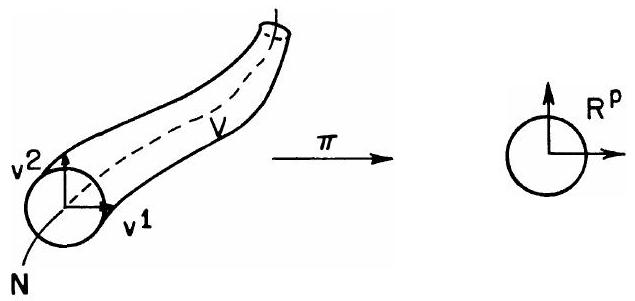
\includegraphics[scale=0.2, center]{2025_05_28_7c9927389b272ddbc2c3g-58}

Figure 18. Constructing a map with given Pontryagin manifold

Now choose a smooth map $\varphi: R^{p} \rightarrow S^{p}$ which maps every $x$ with $\|x\| \geq 1$ into a base point $s_{0}$, and maps the open unit ball in $R^{p}$ diffeomorphically* onto $S^{p}-s_{0}$. Define

$$
f: M \rightarrow S^{p}
$$

by

$$
\begin{array}{lll}
f(x)=\varphi(\pi(x)) & \text { for } & x \varepsilon V \\
f(x)=s_{0} & \text { for } & x \notin V .
\end{array}
$$

Clearly $f$ is smooth, and the point $\varphi(0)$ is a regular value of $f$. Since the corresponding Pontryagin manifold

$$
f^{-1}(\varphi(0))=\pi^{-1}(0)
$$

is precisely equal to the framed manifold $N$, this completes the proof of Theorem C.

In order to prove Theorem B we must first show that the Pontryagin manifold of a map determines its homotopy class. Let $f, g: M \rightarrow S^{p}$ be smooth maps with a common regular value $y$.

Lemma 4. If the framed manifold $\left(f^{-1}(y), f^{*} \mathfrak{v}\right)$ is equal to $\left(g^{-1}(y), g^{*} \mathfrak{v}\right)$, then $f$ is smoothly homotopic to $g$.

Proof. It will be convenient to set $N=f^{-1}(y)$. The hypothesis that $f^{*} \mathfrak{v}=g^{*} \mathfrak{v}$ means that $d f_{x}=d g_{x}$ for all $x \varepsilon N$.

First suppose that $f$ actually coincides with $g$ throughout an entire neighborhood $V$ of $N$. Let $h: S^{p}-y \rightarrow R^{p}$ be stereographic projection. Then the homotopy

$$
\begin{array}{ll}
F(x, t)=f(x) & \text { for } \quad x \in V \\
F(x, t)=h^{-1}[t \cdot h(f(x))+(1-t) \cdot h(g(x))] & \text { for } \quad x \varepsilon M-N
\end{array}
$$

proves that $f$ is smoothly homotopic to $g$.\\
Thus is suffices to deform $f$ so that it coincides with $g$ in some small neighborhood of $N$, being careful not to map any new points into $y$ during the deformation. Choose a product representation

$$
N \times R^{p} \rightarrow V \subset M
$$

for a neighborhood $V$ of $N$, where $V$ is small enough so that $f(V)$ and

\footnotetext{\begin{itemize}
  \item For example, $\varphi(x)=h^{-1}\left(x / \lambda\left(\|x\|^{2}\right)\right)$, where $h$ is the stereographic projection from $s_{0}$ and where $\lambda$ is a smooth monotone decreasing function with $\lambda(t)>0$ for $t<1$ and $\lambda(t)=0$ for $t \geq 1$.
\end{itemize}
}
$g(V)$ do not contain the antipode $\bar{y}$ of $y$. Identifying $V$ with $N \times R^{p}$ and identifying $S^{p}-\bar{y}$ with $R^{p}$, we obtain corresponding mappings
$$
F, G: N \times R^{p} \rightarrow R^{p},
$$
with
$$
F^{-1}(0)=G^{-1}(0)=N \times 0,
$$
and with
$$
d F_{(x, 0)}=d G_{(x, 0)}=\left(\text { projection to } R^{p}\right)
$$
for all $x \in N$.\\
We will first find a constant $c$ so that
$$
F(x, u) \cdot u>0, \quad G(x, u) \cdot u>0
$$
for $x \varepsilon N$ and $0<\|u\|<c$. That is, the points $F(x, u)$ and $G(x, u)$ belong to the same open half-space in $R^{p}$. So the homotopy
$$
(1-t) F(x, u)+t G(x, u)
$$
between $F$ and $G$ will not map any new points into 0 , at least for $\|u\|<c$.\\
By Taylor's theorem
$$
\|F(x, u)-u\| \leq c_{1}\|u\|^{2}, \quad \text { for } \quad\|u\| \leq 1 .
$$

Hence

$$
|(F(x, u)-u) \cdot u| \leq c_{1}\|u\|^{3}
$$

and

$$
F(x, u) \cdot u \geq\|u\|^{2}-c_{1}\|u\|^{3}>0
$$

for $0<\|u\|<\operatorname{Min}\left(c_{1}^{-1}, 1\right)$, with a similar inequality for $G$.\\
To avoid moving distant points we select a smooth map $\lambda: R^{p} \rightarrow R$ with

$$
\begin{array}{ll}
\lambda(u)=1 \quad \text { for } \quad\|u\| \leq c / 2 \\
\lambda(u)=0 \quad \text { for } \quad\|u\| \geq c .
\end{array}
$$

Now the homotopy

$$
F_{t}(x, u)=[1-\lambda(u) t] F(x, u)+\lambda(u) t G(x, u)
$$

deforms $F=F_{0}$ into a mapping $F_{1}$ that (1) coincides with $G$ in the region $\|u\|<c / 2$, (2) coincides with $F$ for $\|u\| \geq c$, and (3) has no new zeros. Making a corresponding deformation of the original mapping $f$, this clearly completes the proof of Lemma 4.

Proof of Theorem B. If $f$ and $g$ are smoothly homotopic, then Lemma 3 asserts that the Pontryagin manifolds $f^{-1}(y)$ and $g^{-1}(y)$ are framed cobordant. Conversely, given a framed cobordism ( $X, \mathfrak{m}$ ) between $f^{-1}(y)$ and $g^{-1}(y)$, an argument completely analogous to the proof of Theorem C constructs a homotopy

$$
F: M \times[0,1] \rightarrow S^{p}
$$

whose Pontryagin manifold ( $F^{-1}(y), F^{*} \mathfrak{v}$ ) is precisely equal to ( $X, \mathfrak{w}$ ). Setting $F_{t}(x)=F(x, t)$, note that the maps $F_{0}$ and $f$ have exactly the same Pontryagin manifold. Hence $F_{0} \sim f$ by Lemma 4; and similarly $F_{1} \sim g$. Therefore $f \sim g$, which completes the proof of Theorem B.

Remarks. Theorems A, B, and C can easily be generalized so as to apply to a manifold $M$ with boundary. The essential idea is to consider only mappings which carry the boundary into a base point $s_{0}$. The homotopy classes of such mappings

$$
(M, \partial M) \rightarrow\left(S^{p}, s_{0}\right)
$$

are in one-one correspondence with the cobordism classes of framed submanifolds

$$
N \subset \operatorname{Interior}(M)
$$

of codimension $p$. If $p \geq \frac{1}{2} m+1$, then this set of homotopy classes can be given the structure of an abelian group, called the $p$-th cohomotopy group $\pi^{p}(M, \partial M)$. The composition operation in $\pi^{p}(M, \partial M)$ corresponds to the union operation for disjoint framed submanifolds of Interior ( $M$ ). (Compare §8, Problem 17.)

\section*{THE HOPF THEOREM}
As an example, let $M$ be a connected and oriented manifold of dimension $m=p$. A framed submanifold of codimension $p$ is just a finite set of points with a preferred basis at each. Let $\operatorname{sgn}(x)$ equal +1 or -1 according as the preferred basis determines the right or wrong orientation. Then $\sum \operatorname{sgn}(x)$ is clearly equal to the degree of the associated map $M \rightarrow S^{m}$. But it is not difficult to see that the framed cobordism class of the 0-manifold is uniquely determined by this integer $\sum \operatorname{sgn}(x)$. Thus we have proved the following.

Theorem of Hopf. If $M$ is connected, oriented, and boundaryless, then two maps $M \rightarrow S^{m}$ are smoothly homotopic if and only if they have the same degree.

On the other hand, suppose that $M$ is not orientable. Then given a basis for $T M_{x}$ we can slide $x$ around $M$ in a closed loop so as to transform the given basis into one of opposite orientation. An easy argument then proves the following:

Theorem. If $M$ is connected but nonorientable, then two maps $M \rightarrow S^{m}$ are homotopic if and only if they have the same mod 2 degree.

The theory of framed cobordism was introduced by Pontryagin in order to study homotopy classes of mappings

$$
S^{m} \rightarrow S^{p}
$$

with $m>p$. For example if $m=p+1 \geq 4$, there are precisely two homotopy classes of mappings $S^{m} \rightarrow S^{p}$. Pontryagin proved this result by classifying framed 1 -manifolds in $S^{m}$. With considerably more difficulty he was able to show that there are just two homotopy classes also in the case $m=p+2 \geq 4$, using framed 2 -manifolds. However, for $m-p>2$ this approach to the problem runs into manifold difficulties.

It has since turned out to be easier to enumerate homotopy classes of mappings by quite different, more algebraic methods.* Pontryagin's construction is, however, a double-edged tool. It not only allows us to translate information about manifolds into homotopy theory; it conversely enables us to translate any information about homotopy into manifold theory. Some of the deepest work in modern topology has come from the interplay of these two theories. René Thom's work on cobordism is an important example of this. (References [36], [21].)

\footnotetext{\begin{itemize}
  \item See for example S.-T. Hu, Homotopy Theory.
\end{itemize}
}\section*{§8. EXERCISES}
In conclusion here are some problems for the reader.\\
Problem 1. Show that the degree of a composition $g \circ f$ is equal to the product (degree $g$ ) (degree $f$ ).

Problem 2. Show that every complex polynomial of degree $n$ gives rise to a smooth map from the Gauss sphere $S^{2}$ to itself of degree $n$.

Problem 3. If two maps $f$ and $g$ from $X$ to $S^{p}$ satisfy $\|f(x)-g(x)\|<2$ for all $x$, prove that $f$ is homotopic to $g$, the homotopy being smooth if $f$ and $g$ are smooth.

Problem 4. If $X$ is compact, show that every continuous map $X \rightarrow S^{p}$ can be uniformly approximated by a smooth map. If two smooth maps $X \rightarrow S^{p}$ are continuously homotopic, show that they are smoothly homotopic.

Problem 5. If $m<p$, show that every map $M^{m} \rightarrow S^{p}$ is homotopic to a constant.

Problem 6. (Brouwer). Show that any map $S^{n} \rightarrow S^{n}$ with degree different from $(-1)^{n+1}$ must have a fixed point.

Problem 7. Show that any map $S^{n} \rightarrow S^{n}$ of odd degree must carry some pair of antipodal points into a pair of antipodal points.

Problem 8. Given smooth manifolds $M \subset R^{k}$ and $N \subset R^{l}$, show that the tangent space $T(M \times N)_{(x, y)}$ is equal to $T M_{x} \times T N_{y}$.

Problem 9. The graph $\Gamma$ of a smooth map $f: M \rightarrow N$ is defined to be the set of all $(x, y) \varepsilon M \times N$ with $f(x)=y$. Show that $\Gamma$ is a smooth\\
manifold and that the tangent space

$$
T \Gamma_{(x, y)} \subset T M_{x} \times T N_{y}
$$

is equal to the graph of the linear map $d f_{x}$.\\
Problem 10. Given $M \subset R^{k}$, show that the tangent bundle space

$$
T M=\left\{(x, v) \varepsilon M \times R^{k} \mid v \varepsilon T M_{x}\right\}
$$

is also a smooth manifold. Show that any smooth map $f: M \rightarrow N$ gives rise to a smooth map

$$
d f: T M \rightarrow T N
$$

where

$$
d \text { (identity) }=\text { identity }, \quad d(g \circ f)=(d g) \circ(d f) .
$$

Problem 11. Similarly show that the normal bundle space

$$
E=\left\{(x, v) \varepsilon M \times R^{k} \mid v \perp T M_{x}\right\}
$$

is a smooth manifold. If $M$ is compact and boundaryless, show that the correspondence

$$
(x, v) \mapsto x+v
$$

from $E$ to $R^{k}$ maps the $\epsilon$-neighborhood of $M \times 0$ in $E$ diffeomorphically onto the $\epsilon$-neighborhood $N_{\epsilon}$ of $M$ in $R^{k}$. (Compare the Product Neighborhood Theorem in §7.)

Problem 12. Define $r: N_{\epsilon} \rightarrow M$ by $r(x+v)=x$. Show that $r(x+v)$ is closer to $x+v$ than any other point of $M$. Using this retraction $r$, prove the analogue of Problem 4 in which the sphere $S^{p}$ is replaced by a manifold $M$.

Problem 13. Given disjoint manifolds $M, N \subset R^{k+1}$, the linking map

$$
\lambda: M \times N \rightarrow S^{k}
$$

is defined by $\lambda(x, y)=(x-y) /\|x-y\|$. If $M$ and $N$ are compact, oriented, and boundaryless, with total dimension $m+n=k$, then the degree of $\lambda$ is called the linking number $l(M, N)$. Prove that

$$
l(N, M)=(-1)^{(m+1)(n+1)} l(M, N) .
$$

If $M$ bounds an oriented manifold $X$ disjoint from $N$, prove that $l(M, N)=0$. Define the linking number for disjoint manifolds in the sphere $S^{m+n+1}$.

Problem 14, The Hopf Invariant. If $y \neq z$ are regular values for a map $f: S^{2 p-1} \rightarrow S^{p}$, then the manifolds $f^{-1}(y), f^{-1}(z)$ can be oriented as in §5; hence the linking number $l\left(f^{-1}(y), f^{-1}(z)\right)$ is defined.\\
a) Prove that this linking number is locally constant as a function of $y$.\\
b) If $y$ and $z$ are regular values of $g$ also, where

$$
\|f(x)-g(x)\|<\|y-z\|
$$

for all $x$, prove that

$$
l\left(f^{-1}(y), f^{-1}(z)\right)=l\left(g^{-1}(y), f^{-1}(z)\right)=l\left(g^{-1}(y), g^{-1}(z)\right) .
$$

c) Prove that $l\left(f^{-1}(y), f^{-1}(z)\right)$ depends only on the homotopy class of $f$, and does not depend on the choice of $y$ and $z$.

This integer $H(f)=l\left(f^{-1}(y), f^{-1}(z)\right)$ is called the Hopf invariant of $f$. (Reference [15].)

Problem 15. If the dimension $p$ is odd, prove that $H(f)=0$. For a composition

$$
S^{2 p-1} \xrightarrow{f} S^{p} \xrightarrow{g} S^{p}
$$

prove that $H(g \circ f)$ is equal to $H(f)$ multiplied by the square of the degree of $g$.

The Hopf fibration $\pi: S^{3} \rightarrow S^{2}$ is defined by

$$
\pi\left(x_{1}, x_{2}, x_{3}, x_{4}\right)=h^{-1}\left(\left(x_{1}+i x_{2}\right) /\left(x_{3}+i x_{4}\right)\right)
$$

where $h$ denotes stereographic projection to the complex plane. Prove that $H(\pi)=1$.

Problem 16. Two submanifolds $N$ and $N^{\prime}$ of $M$ are said to intersect transversally if, for each $x \varepsilon N \cap N^{\prime}$, the subspaces $T N_{x}$ and $T N_{x}^{\prime}$ together generate $T M_{x}$. (If $n+n^{\prime}<m$ this means that $N \cap N^{\prime}=\varnothing$.) If $N$ is a framed submanifold, prove that it can be deformed slightly so as to intersect a given $N^{\prime}$ transversally. Prove that the resulting intersection is a smooth manifold.

Problem 17. Let $\Pi^{p}(M)$ denote the set of all framed cobordism classes of codimension $p$ in $M$. Use the transverse intersection operation to define a correspondence

$$
\Pi^{p}(M) \times \Pi^{q}(M) \rightarrow \Pi^{p+q}(M)
$$

If $p \geq \frac{1}{2} m+1$, use the disjoint union operation to make $\Pi^{p}(M)$ into an abelian group. (Compare p. 50.)

\section*{APPENDIX CLASSIFYING 1-MANIFOLDS}
We will prove the following result, which has been assumed in the text. A brief discussion of the classification problem for higher dimensional manifolds will also be given.

Theorem. Any smooth, connected 1-dimensional manifold is diffeomorphic either to the circle $S^{1}$ or to some interval of real numbers.\\
(An interval is a connected subset of $R$ which is not a point. It may be finite or infinite; closed, open, or half-open.)

Since any interval is diffeomorphic* either to $[0,1],(0,1]$, or $(0,1)$, it follows that there are only four distinct connected 1 -manifolds.

The proof will make use of the concept of "arc-length." Let $I$ be an interval.

Definition. A map $f: I \rightarrow M$ is a parametrization by arc-length if $f$ maps $I$ diffeomorphically onto an open subset $\dagger$ of $M$, and if the "velocity vector" $d f_{s}(1) \varepsilon T M_{f(s)}$ has unit length, for each $s \varepsilon I$.

Any given local parametrization $I^{\prime} \rightarrow M$ can be transformed into a parametrization by arc-length by a straightforward change of variables.

Lemma. Let $f: I \rightarrow M$ and $g: J \rightarrow M$ be parametrizations by arc-length. Then $f(I) \cap g(J)$ has at most two components. If it has only one component, then $f$ can be extended to a parametrization by arc-length of the union $f(I) \cup g(J)$. If it has two components, then $M$ must be diffeomorphic to $S^{1}$.

\footnotetext{\begin{itemize}
  \item For example, use a diffeomorphism of the form
\end{itemize}

$$
f(t)=a \tanh (t)+b
$$

$\dagger$ Thus $I$ can have boundary points only if $M$ has boundary points.
}Proof. Clearly $g^{-1}$ of maps some relatively open subset of $I$ diffeomorphically onto a relatively open subset of $J$. Furthermore the derivative of $g^{-1} \circ f$ is equal to $\pm 1$ everywhere.

Consider the graph $\Gamma \subset I \times J$, consisting of all $(s, t)$ with $f(s)=g(t)$. Then $\Gamma$ is a closed subset of $I \times J$ made up of line segments of slope $\pm 1$. Since $\Gamma$ is closed and $g^{-1} \circ f$ is locally a diffeomorphism, these line segments cannot end in the interior of $I \times J$, but must extend to the boundary. Since $g^{-1} \circ f$ is one-one and single valued, there can be at most one of these segments ending on each of the four edges of the rectangle $I \times J$. Hence $\Gamma$ has at most two components. (See Figure 19.) Furthermore, if there are two components, the two must have the same slope.\\
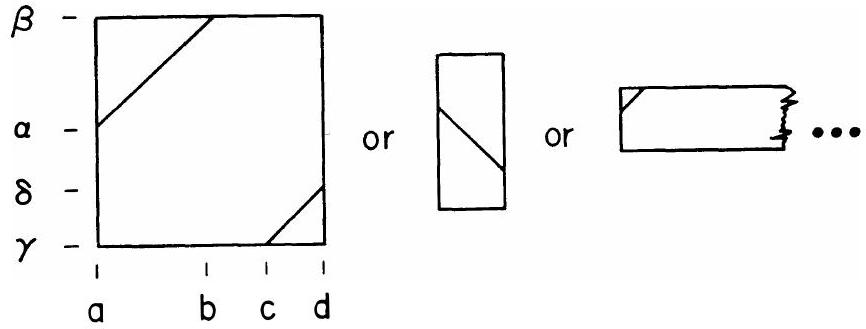
\includegraphics[scale=0.2, center]{2025_05_28_7c9927389b272ddbc2c3g-67}

Figure 19. Three of the possibilities for $\Gamma$

If $\Gamma$ is connected, then $g^{-1} \circ f$ extends to a linear map $L: R \rightarrow R$. Now $f$ and $g \circ L$ piece together to yield the required extension

$$
F: I \cup L^{-1}(J) \rightarrow f(I) \cup g(J) .
$$

If $\Gamma$ has two components, with slope say +1 , they must be arranged as in the left-hand rectangle of Figure 19. Translating the interval $J=(\gamma, \beta)$ if necessary, we may assume that $\gamma=c$ and $\delta=d$, so that

$$
a<b \leq c<d \leq \alpha<\beta .
$$

Now setting $\theta=2 \pi t /(\alpha-a)$, the required diffeomorphism

$$
h: S^{1} \rightarrow M
$$

is defined by the formula

$$
\begin{aligned}
h(\cos \theta, \sin \theta) & =f(t) \quad \text { for } \quad a<t<d, \\
& =g(t) \quad \text { for } \quad c<t<\beta .
\end{aligned}
$$

The image $h\left(S^{1}\right)$, being compact and open in $M$, must be the entire manifold $M$. This proves the lemma.

Proof of Classification Theorem. Any parametrization by arclength can be extended to one

$$
f: I \rightarrow M
$$

which is maximal in the sense that $f$ cannot be extended over any larger interval as a parametrization by arc-length: it is only necessary to extend $f$ as far as possible to the left and then as far as possible to the right.

If $M$ is not diffeomorphic to $S^{1}$, we will prove that $f$ is onto, and hence is a diffeomorphism. For if the open set $f(I)$ were not all of $M$, there would be a limit point $x$ of $f(I)$ in $M-f(I)$. Parametrizing a neighborhood of $x$ by arc-length and applying the lemma, we would see that $f$ can be extended over a larger interval. This contradicts the assumption that $f$ is maximal and hence completes the proof.

Remarks. For manifolds of higher dimension the classification problem becomes quite formidable. For 2-dimensional manifolds, a thorough exposition has been given by Kerékjártó [17]. The study of 3-dimensional manifolds is very much a topic of current research. (See Papakyriakopoulos [26].) For compact manifolds of dimension $\geq 4$ the classification problem is actually unsolvable.* But for high dimensional simply connected manifolds there has been much progress in recent years, as exemplified by the work of Smale [31] and Wall [37].

\footnotetext{\begin{itemize}
  \item See Markov [19]; and also a forthcoming paper by Boone, Haken, and Poénaru in Fundamenta Mathematicae.
\end{itemize}
}\section*{BIBLIOGRAPHY}
The following is a miscellaneous list consisting of original sources and of recommended textbooks. For the reader who wishes to pursue the study of differential topology, let me recommend Milnor [22], Munkres [25], and Pontryagin [28]. The survey articles [23] and [32] should also prove useful. For background knowledge in closely related fields, let me recommend Hilton and Wylie [11], Hu [16], Lang [18], de Rham [29], Steenrod [34], and Sternberg [35].\\[0pt]
[1] Allendoerfer, C. B., "The Euler number of a Riemann manifold," Amer. Jour. Math. 62 (1940), 243-248.\\[0pt]
[2] Apostol, T. M., Mathematical Analysis. Reading, Mass.: Addison-Wesley, 1957.\\[0pt]
[3] Auslander, L., and R. MacKenzie, Introduction to Differentiable Manifolds. New York: McGraw-Hill, 1963.\\[0pt]
[4] Brouwer, L. E. J., "Uber Abbildung von Mannigfaltigkeiten", Math. Annalen 71 (1912), 97-115.\\[0pt]
[5] Brown, A. B., "Functional dependence," Trans. Amer. Math. Soc. 38 (1935), 379-394. (See Theorem 3-III.)\\[0pt]
[6] Chern, S. S., "A simple intrinsic proof of the Gauss-Bonnet formula for closed Riemannian manifolds," Annals of Math. 45 (1944), 747-752.\\[0pt]
[7] Dieudonné, J., Foundations of Modern Analysis. New York: Academic Press, 1960.\\[0pt]
[8] Dubovickiǐ, A. Ya., "On differentiable mappings of an $n$-dimensional cube into a $k$-dimensional cube," Mat. Sbornik N.S. 32 (74), (1953), 443-464. (In Russian.)\\[0pt]
[9] Fenchel, W., "On total curvatures of Riemannian manifolds," Jour. London Math. Soc. 15 (1940), 15-22.\\[0pt]
[10] Goffman, C., Calculus of Several Variables. New York: Harper \& Row, 1965.\\[0pt]
[11] Hilton, P., and S. Wylie, Homology Theory. Cambridge Univ. Press, 1960.\\[0pt]
[12] Hirsch, M., "A proof of the nonretractibility of a cell onto its boundary," Proc. Amer. Math. Soc. 14 (1963), 364-365.\\[0pt]
[13] Hopf, H., "Abbildungsklassen $n$-dimensionaler Mannigfaltigkeiten," Math. Annalen 96 (1926), 209-224.\\[0pt]
[14] -, "Vektorfelder in n-dimensionalen Mannigfaltigkeiten," Math. Annalen 96 (1926), 225-250.\\[0pt]
[15] —, "Uber die Abbildungen von Sphären auf Sphären niedrigerer Dimension," Fundamenta Mathematicae 25 (1935), 427-440.\\[0pt]
[16] Hu, S.-T., Homotopy Theory. New York: Academic Press, 1959.\\[0pt]
[17] Kerékjártó, B. v., Vorlesungen über Topologie. Berlin: Springer, 1923.\\[0pt]
[18] Lang, S., Introduction to Differentiable Manifolds. New York: Interscience, 1962.\\[0pt]
[19] Markov, A. A., "Insolubility of the problem of homeomorphy," Proceedings Intern. Congress of Math. 1958, Cambridge Univ. Press, 1960, pp. 300-306. (In Russian.)\\[0pt]
[20] Milnor, J., "On manifolds homeomorphic to the 7 -sphere," Annals of Math. 64 (1956), 399-405.\\[0pt]
[21] -, "A survey of cobordism theory," L'Enseignement math. 8 (1962), 16-23.\\[0pt]
[22] --, Morse Theory. (Annals Studies 51.) Princeton Univ. Press, 1963.\\[0pt]
[23] -, "Differential topology," Lectures on Modern Mathematics, II, ed. T. L. Saaty, New York: Wiley, 1964, pp. 165-183.\\[0pt]
[24] Morse, A. P., "The behavior of a function on its critical set," Annals of Math. 40 (1939), 62-70.\\[0pt]
[25] Munkres, J. R., Elementary Differential Topology. (Annals Studies 54). Princeton Univ. Press, 1963.\\[0pt]
[26] Papakyriakopoulos, C. D., "The theory of three-dimensional manifolds since 1950," Proceedings Intern. Congress of Math. 1958, Cambridge Univ. Press, 1960, pp. 433-440.\\[0pt]
[27] Pontryagin, L. S., "A classification of continuous transformations of a complex into a sphere," Doklady Akad. Nauk. S.S.S.R. (Comptes Rendues) 19 (1938), 147-149.\\[0pt]
[28] -, "Smooth manifolds and their applications in homotopy theory," Amer. Math. Soc. Translations, Ser. 2, II (1959), 1-114. (Translated from Trudy Inst. Steklov 45 (1955).)\\[0pt]
[29] Rham, G. de, Variétés différentiables. Paris: Hermann, 1955.\\[0pt]
[30] Sard, A., "The measure of the critical points of differentiable maps," Bull. Amer. Math. Soc. 48 (1942), 883-890.\\[0pt]
[31] Smale, S., "Generalized Poincaré's conjecture in dimensions greater than four," Annals of Math. 74 (1961), 391-406.\\[0pt]
[32] -, "A survey of some recent developments in differential topology," Bull. Amer. Math. Soc. 69 (1963), 131-145.\\[0pt]
[33] Spivak, M., Calculus on Manifolds. New York: Benjamin, 1965.\\[0pt]
[34] Steenrod, N., The Topology of Fibre Bundles. Princeton Univ. Press, 1951.\\[0pt]
[35] Sternberg, S., Lectures on Differential Geometry. New York: PrenticeHall, 1964.\\[0pt]
[36] Thom, R., "Quelques propriétés globales des variétés différentiables," Commentarii Math. Helvet. 28 (1954), 17-86.\\[0pt]
[37] Wall, C. T. C., "Classification of ( $n-1$ )-connected $2 n$-manifolds," Annals of Math. 75 (1962), 163-189.\\[0pt]
[38] Whitney, H., "A function not constant on a connected set of critical points," Duke Math. Jour. 1 (1935), 514-517.

\section*{PAGE-BARBOUR LECTURE SERIES}
The Page-Barbour Lecture Foundation was founded in 1907 by a gift from Mrs. Thomas Nelson Page (née Barbour) and the Honorable Thomas Nelson Page for the purpose of bringing to the University of Virginia each session a series of lectures by an eminent person in some field of scholarly endeavor. The materials in this volume were presented by Professor John W. Milnor in December, 1963, as the forty-seventh series sponsored by the Foundation.

\section*{INDEX}
antipodal map, 30, 52\\
boundary, 12\\
Brouwer, L. E. J., 35, 52\\
degree, 20, 28\\
fixed point theorem, 14\\
Brown, A. B., 10, 11\\
chain rule for derivatives, 3,7\\
cobordism, 42, 43, 51\\
codimension, 42\\
cohomotopy, 50\\
coordinate system, 1\\
corresponding vector fields, 32\\
critical point, 8, 11\\
critical value, 8,11\\
degree of a map, 28\\
mod two, 20\\
derivative of a map, 2-7\\
diffeomorphism, 1\\
differential topology, 1, 59\\
dimension of a manifold, 1, 5, 7\\
disk, 13, 14\\
Euler number, 35, 36, 40\\
framed cobordism, 43\\
framed submanifold, 42, 44, 46\\
Fubini theorem, 17\\
fundamental theorem of algebra, 8\\
Gauss-Bonnet theorem, 38\\
Gauss mapping, 35, 38\\
half-space, 12\\
Hirsch, M., 14\\
homotopy, 20, 21, 52\\
Hopf, H., 31, 35, 36, 40, 51, 54\\
index (of a zero of a vector field), 3234\\
index sum, 35-41\\
inverse function theorem, 4,8\\
inward vector, 26\\
isotopy, 21, 22, 34\\
linking, 53\\
Morse, A. P., 10\\
Morse, M., 40\\
nondegenerate zero (of a vector field) 37, 40\\
normal bundle, 53\\
normal vectors, 11, 12, 42\\
orientation, 26\\
of a boundary, 27\\
of $F^{-1}(y), 28$\\
outward vector, 26\\
parametrization, 1, 2\\
by arc-length, 55\\
Poincaré, H., 35\\
Pontryagin, L., 16, 42\\
Pontryagin manifold, 43\\
product neighborhood theorem, 46\\
regular point, 7\\
regular value, $8,11,13,14,20,27,40,43$\\
Sard, A., 10, 16\\
smooth manifolds, 1\\
with boundary, 12\\
smooth manifolds (cont.)\\
the classification problem, 57\\
of dimension zero, 2\\
of dimension one, 14, 55\\
oriented, 26\\
smooth maps (= smooth mappings), 1\\
sphere, 2\\
stereographic projection, 9, 48\\
tangent bundle, 53\\
tangent space, 2-5\\
at a boundary point, 12, 26\\
tangent vector, 2\\
vector fields, 30, 32-41\\
Weierstrass approximation theorem, 14

\section*{INDEX OF SYMBOLS}
$\operatorname{deg}(f ; y), \quad 27$\\
$d f_{x}$, 2-7\\
$D^{m}, \quad 14$\\
$\partial X, 12$\\
$f^{*} \mathfrak{v}, \quad 43$\\
$\# f^{-1}(y), \quad 8$\\
$g \circ f, \quad 1$\\
$H^{m}, \quad 12$\\
$R^{k}, 1$\\
$S^{n-1}, \quad 2$\\
$T M_{x}, \quad 2-5$\\
$\|x\|, \quad 14$

\section*{TOPOLOGY FROM THE DIFFERENTIABLE VIEWPOINT}
was composed and printed by\\
The William Byrd Press, Inc., Richmond, Virginia and bound by Russell Rutter Co., Inc., New York, N. Y.\\
The types are Modern Number 8 and Century Schoolbook, and the paper is Oxford's Bookbuilders Plate.\\
Design is by Edward Foss.

\begin{itemize}
  \item 
\end{itemize}

\begin{itemize}
  \item 
\end{itemize}

\begin{itemize}
  \item 
\end{itemize}

\begin{itemize}
  \item 
\end{itemize}

\begin{itemize}
  \item 
\end{itemize}

\begin{itemize}
  \item 
\end{itemize}

\begin{itemize}
  \item 
\end{itemize}

\begin{itemize}
  \item 
\end{itemize}

\begin{itemize}
  \item 
\end{itemize}

\begin{itemize}
  \item 
\end{itemize}

\begin{itemize}
  \item 
\end{itemize}

\begin{itemize}
  \item 
\end{itemize}

\begin{itemize}
  \item 
\end{itemize}

\begin{itemize}
  \item 
\end{itemize}

\begin{itemize}
  \item 
\end{itemize}

\begin{itemize}
  \item 
\end{itemize}

\begin{itemize}
  \item 
\end{itemize}


\end{document}